%*******************************************************************************
%******************************* Final Chapter *********************************
%*******************************************************************************

\chapter{Cosmic Muon Tomography at Wylfa}\label{chp:cosmicMuonTomography}

\ifpdf
    \graphicspath{{Chapter5/Figs/Raster/}{Chapter5/Figs/PDF/}{Chapter5/Figs/}}
\else
    \graphicspath{{Chapter5/Figs/Vector/}{Chapter5/Figs/}}
\fi

This chapter will focus on cosmic muon tomography using data collected the deployment at the Wylfa nuclear power plant. This will include the analysis techniques used to extract the data from the detector. Then the deployment at Wylfa will be covered including the distributions of $\phi$ and $\theta$ and any deficits in the cosmic muon incidence that would indicate buildings (referred to as ``shadows''). These shadows are then compared to simulated approximations of the reactor buildings in GEANT4. The outlines expected from each component of the simulated reactor site produce a composite shadow shape that matches measured data extremely well. Then the uncertainties relating to the cosmic muon tracker's reconstruction of $\phi$ and $\theta$ are quantified. Finally, simulated cosmic ray data using a realistic distribution from the CRY library is used to assess the validity of the cosmic muon data taken at Wylfa and the control data from Liverpool. 

\section{Deployment At Wylfa}\label{sec:deploymentAtWylfa}
The detector was deployed at the Wylfa Nuclear power station from June 2014 to February 2016 with data being taken continuously over that time period both with the reactor on and reactor off taking the IBD measurements \cite{Carroll_2018} (figure \ref{fig:prototypeMeasumentFlux}). The placement of the detector in relation to the Wylfa site buildings can be seen in figure \ref{subFig:DetectorPositionTopDown}, the reactors are located at either end of the ``dog bone''-shaped main reactor building and are assumed to be in the centre of the cylinders. Whilst there is no good height data for the buildings at the Wylfa reactor site publicly available there is a drone picture available seen in figure \ref{subFig:wylfaArielView}. In figure \ref{subFig:wylfaArielView} the tallest buildings are clearly visible, of particular importance are the main reactor building and the turbine hall (the long building running the length of the reactor building). The service buildings in between the turbine hall and the  main reactor building are also very important as they are much closer to the detector's position as seen in figure \ref{subFig:DetectorPositionTopDown} and so will appear taller than the main reactor building. Also shown in figures \ref{subFig:DetectorPositionTopDown} and \ref{subFig:wylfaArielView} are the steam bridges that connect the main reactor building and the turbine hall. The steam bridges are not large buildings and are approximated to be 5\,m wide in z and 10\,m off of the ground in simulation. One of the steam bridges is very close to the detector as can be seen in figure \ref{subFig:DetectorPositionTopDown} and so will occlude a significant portion of the incident muon flux the detector observes. 

\begin{figure}[!h]
\centering
\begin{subfigure}{.5\textwidth}
  \centering
  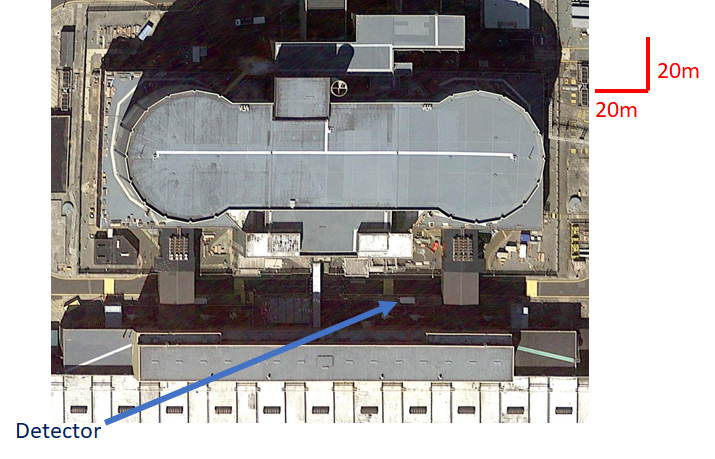
\includegraphics[width=\linewidth]{Chapter5/Figs/wylfaRasterNew/DetectorPositionTopDown.png}
  \captionsetup{width=.9\linewidth}
  \caption{}
  \label{subFig:DetectorPositionTopDown}
\end{subfigure}%
\begin{subfigure}{.5\textwidth}
  \centering
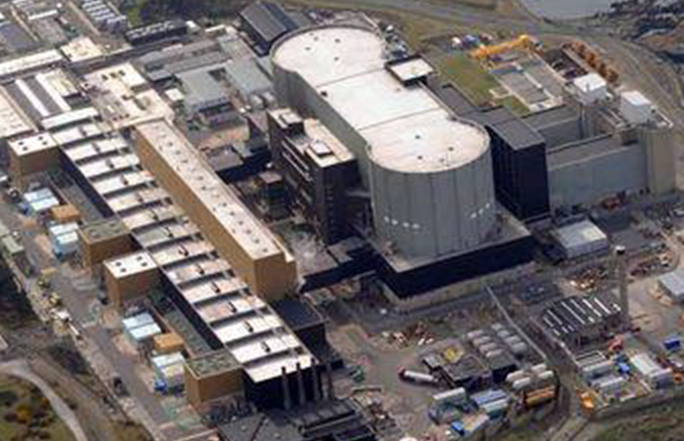
\includegraphics[width=\linewidth]{Chapter5/Figs/Raster/wylfaArielView.png}
  \captionsetup{width=.9\linewidth}
  \caption{}
  \label{subFig:wylfaArielView}
\end{subfigure}
\caption[Aerial views of the Wylfa reactor site.]{The Wylfa reactor site. (a) shows a Google Maps aerial photography image, displaying the approximate detector position. The detector is in the middle of many site buildings occluding the incident cosmic rays \cite{GoogleMapsWylfaLink}. (b) An aerial view of the Wylfa power station the main reactor building is the shape of a "dog bone" the detector was placed in-between the turbine hall and reactor building (the turbine hall is the long building running the length of the reactor building). Edited from \cite{wylfaDronePictureLink}.}
\label{fig:DetectorPosition_TopDownAndAriel}
\end{figure}

% \begin{figure}[!h]
%  \centering
%  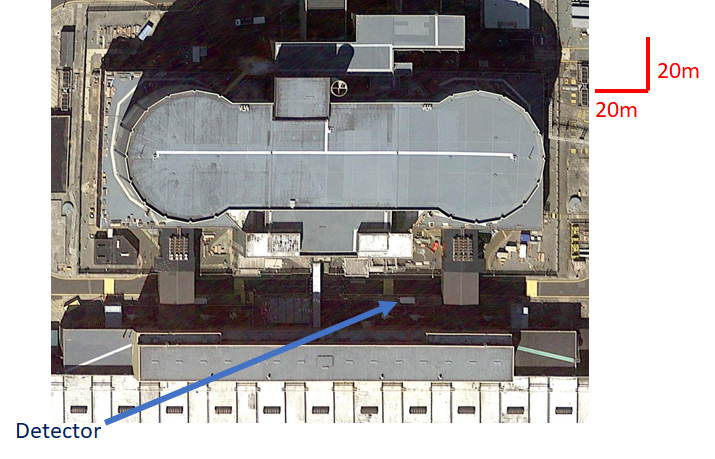
\includegraphics[width=0.75\linewidth]{Chapter5/Figs/wylfaRasterNew/DetectorPositionTopDown.png}
%  \captionof{figure}{Google Maps aerial photography image, displaying the Wylfa reactor site as well as the approximate detector position. The detector is in the middle of many site buildings occluding the incident cosmic rays. Key buildings shown are the reactor building, the turbine hall and the steam pipe connections between the two \cite{GoogleMapsWylfaLink}.} 
%  \label{fig:DetectorPositionTopDown}
% \end{figure}

% \begin{figure}[!h]
%  \centering
%  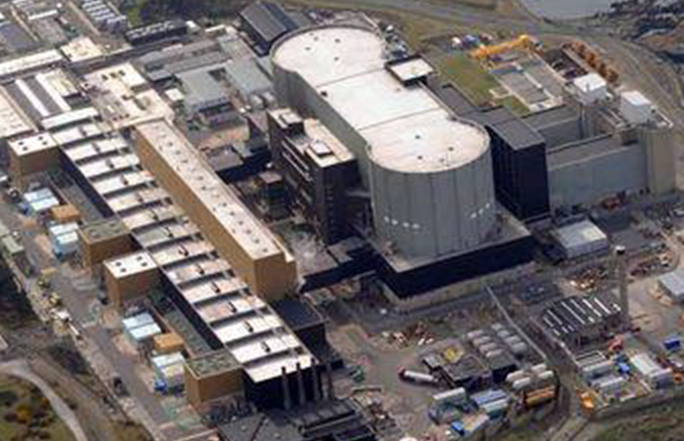
\includegraphics[width=0.6\linewidth]{Chapter5/Figs/Raster/wylfaArielView.png}
%  \captionof{figure}{An aerial view of the Wylfa power station the main reactor building is the shape of a "dog bone" the detector was placed in-between the turbine hall and reactor building. Edited from \cite{wylfaDronePictureLink}.} 
%  \label{fig:wylfaAir}
% \end{figure}

In addition, the composition of these buildings needs to be considered as well. The structure of the reactor building is seen in figure \ref{fig:wylfaReactorRoughStructure} with the top half of the structure being air wrapped in a concrete shell and the bottom half having thick concrete shielding. As a result, any cosmic muons that traverse through the top of the structure will have a much greater chance to penetrate than those traversing it at lower angles of $\theta$. This means that the top portions of the buildings will be ``blurred'' to some extent as the amount of material will be initially low. Secondly, it will mean that the transmission value will decrease with the $\theta$ value. This decrease will be especially pronounced where the reactor core and reactor shielding are located. 

\begin{figure}[!h]
 \centering
 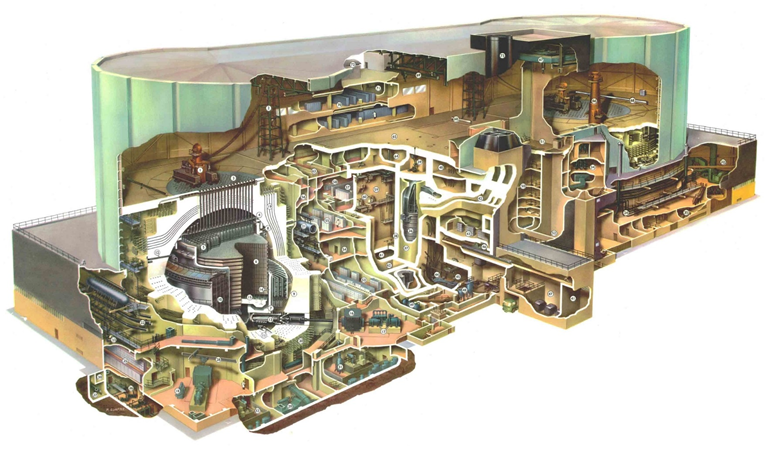
\includegraphics[width=0.7\linewidth]{Chapter5/Figs/wylfaRasterNew/wylfaReactorRoughStructure.png}
 \captionof{figure}[A cutaway diagram of the Wylfa reactor buildings.]{A cutaway diagram from \cite{neiMag_1965}. Shows the internal structure of the Wylfa reactor buildings from the back. The bottom half of the reactor buildings have thick concrete walls whilst the upper section is mostly storage. As this is a qualitative illustration of the building for public communication, the exact details, locations of features and proportions may not match the exact physical structure.} 
 \label{fig:wylfaReactorRoughStructure}
\end{figure}

\section{Initial Data Processing And Selection Criteria}\label{sec:muonAnalysisChain}
In order to analyse the muon data from the Wylfa deployment analysis chains are required. One of the chains used is based on the T2K analysis chain which converts the data stored in MIDAS \cite{ritt1997midas} files (\texttt{.mid.gz} files) to ROOT Ntuples (\texttt{.root} files) and calibrates the data using special calibration runs (``pedestal files''). The second analysis chain is designed to analyse the simulated files and data from the upgraded detector once it is complete. However, because the new analysis chain is multi-threaded and much faster than the original chain (and independent of a specific operating system kernel, specific ROOT version and specific GEANT4 version) it is preferable to use the new analysis chain for the prototype detector data as well. This also has the advantage of ensuring the cosmic muon tracker developed in section \ref{sec:SimulationOfCosmics} will be functional for both versions of the detector, allowing for a direct comparison once the VIDARR detector upgrade is complete. 
\\\\The detector deployed at Wylfa analysed data in cycles of 1.5\,$\mathrm{\mu}$s. There are 23 cycles in the data indexed 0 -- 22 with cycle 18 as the trigger cycle and cycles 17 and 19 considered to be underflow and overflow for the trigger signal respectively. The cycles are then interpreted depending on whether the user wants to analyse cosmic muon data or IBD data. For cosmic muon data each cycle will be considered as its own event with trigger cycles 17 -- 19 being ignored. For IBD analysis, the data is split between prompt (cycles 0 -- 16) and delayed (cycles 17 -- 19) with the post-trigger data (cycles 20 -- 22) being ignored (see figure \ref{fig:CycleExplaination}). The mode is determined by the program \texttt{convertOldDetectorData} to ensure subsequent programs in the analysis chain can interpret the data correctly. Simulated data requires minimal changes as it classifies data into delayed, prompt, and ambiguous categories automatically using information based on particle generation.
% Unfortunately, due to the COVID-19 pandemic, the upgraded detector remains incomplete and so the calibration program for the new detector data has not been constructed at present. 

\begin{figure}[!h]
 \centering
 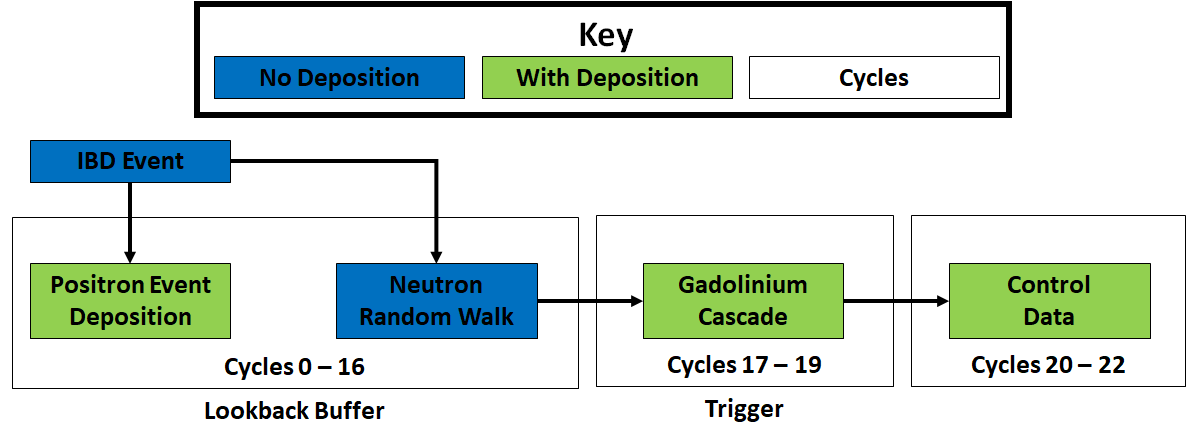
\includegraphics[width=\linewidth]{Chapter6/Figs/CycleExplaination.png}
 \captionof{figure}[The prototype detector's timing cycles.]{The prototype's cycles. The trigger signal is the neutron induced gadolinium cascade in cycle 18 cycles 17 and 19 are trigger overflow. Cycles 0-16 are observed for any signs of a positron cluster as a lookback buffer. Cycles 20-22 contain control information.} 
 \label{fig:CycleExplaination}
\end{figure}

% The cosmic muon events at Wylfa were taken in accidental coincidence and as a result, much noise made it into the cosmic muon data sets. 
Cosmic muon events are large events that resemble the Gd cascade trigger signal in size. As a result, a muon veto was developed in the prototype that observes the edge of each side and checks for concurrent hits. If concurrent hits are found then the event is considered cosmic and therefore discarded. This is done via the TFB electronics. However, this veto does not exclude all cosmic muon events. Some cosmic muon events skip over bars if they are angled properly and as a result they are included in the data set. This is referred to as ``Accidental coincidence.'' For the Wylfa deployment there was no dedicated cosmic muon mode. All cosmic muon events were therefore taken in accidental coincidence. As a result, background rates for the cosmic muon data are high and require additional pre-processing to remove events unsuitable for tracker-based analysis. In the raw unprocessed data sets for every 3 cosmic muon events, there are $\sim$ 10000 noise events. As such the SVM machine learning technique previously described in section \ref{sec:MachineLearningTrigger} was used to reject background. It found the best separating hyperplane at eight bars when using a threshold of 17.325\,PE (0.693\,MeV) (figure \ref{fig:cosmic8BarSignalNoiseCutSVM}). In figure \ref{fig:cosmic8BarSignalNoiseCutSVM} most of the background is highly concentrated at a low number of bar hits. Therefore, the simple 8 bar cut seems intuitively correct. This cut removes 99.9\,\% of background and keeps 99\,\% of the cosmic muon signal so now for every three cosmic events there are approximately 10 noise events. The signal-to-background ratio has therefore improved from $\sim$ 3:10000 to $\sim$ 3:10, keeping almost all the signal. These numbers are summarised in table \ref{tab:snRatioSvm}. Finding simple effective selection criteria is a task SVMs are well suited to making it very useful as a data quality tool. 

\begin{table*}[!h]
\centering
\begin{tabular}{lccc}  
\toprule
Processing stage & Remaining Background\,[\%] & Remaining Signal\,[\%] & Signal-to-background \\
\midrule
Raw Data         & 100                        & 100             & $\sim$ 3:10000\\
Data Past SVM    & $\sim$ 0.1                 & $\sim$ 99       & $\sim$ 3:10\\
\bottomrule  
\end{tabular}
\caption{A table showing how the data quality requirements determined by a SVM where all events that have < 8 bars hit < 0.693\,MeV are removed. Despite the simple selection criteria the signal-to-background ratio greatly improves.}
\label{tab:snRatioSvm}
\end{table*}

\begin{figure}[!h]
\centering
\begin{subfigure}{.5\textwidth}
  \centering
  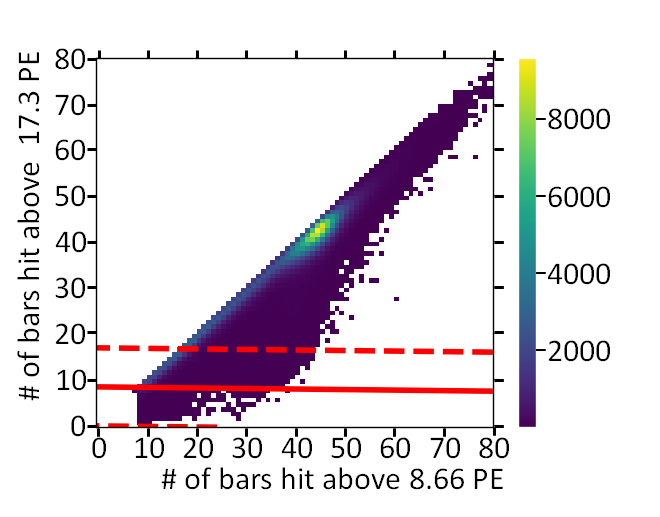
\includegraphics[width=\linewidth]{Chapter6/Figs/Raster/Cosmic8BarSignalCutSvmMedText.png}
  \captionsetup{width=.9\linewidth}
  \caption{}
  \label{subFig:cosmic8BarSignalCutSVM}
\end{subfigure}%
\begin{subfigure}{.5\textwidth}
  \centering
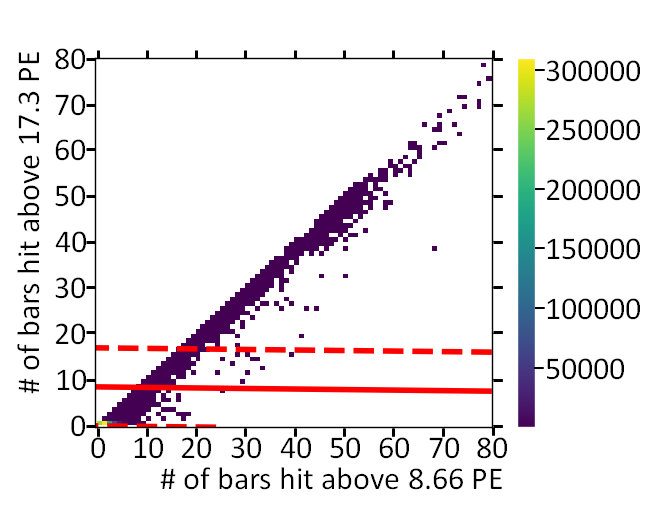
\includegraphics[width=\linewidth]{Chapter6/Figs/Raster/Cosmic8BarNoiseCutSvmMedText.png}
  \captionsetup{width=.9\linewidth}
  \caption{}
  \label{subFig:cosmic8BarNoiseCutSVM}
\end{subfigure}
\caption[An SVM classifier separating cosmic signal from noise.]{How an SVM classifier separates out measured cosmic muon data. It settled on an 8 bar cut with a threshold of 17\,PE (0.68\,MeV). Where everything above the solid line is considered a cosmic muon and everything below is considered noise. In (a) the muon data is represented. In (b) the noise data is represented. The logic for the SVM classifier is outlined in section \ref{sec:MachineLearningTrigger}.}
\label{fig:cosmic8BarSignalNoiseCutSVM}
\end{figure}

% \begin{figure}[!h]
% \centering
% \begin{subfigure}{.5\textwidth}
%   \centering
%   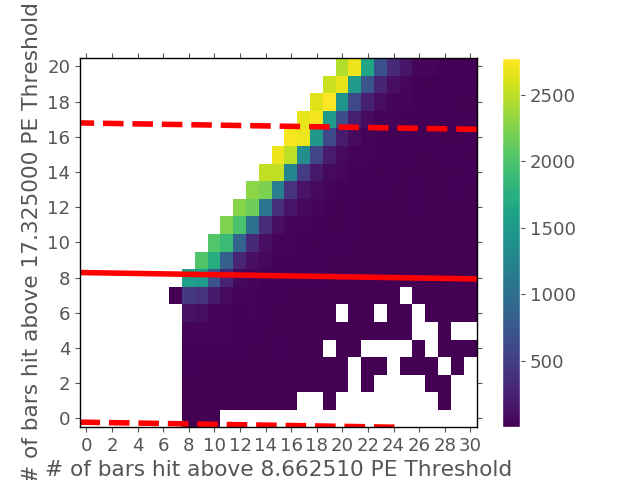
\includegraphics[width=\linewidth]{Chapter5/Figs/Raster/Cosmic8BarSignalZoomCutSVM.png}
%   \captionsetup{width=.9\linewidth}
%   \caption{} 
%   \label{subFig:cosmic8BarSignalZoomCutSVM}
% \end{subfigure}%
% \begin{subfigure}{.5\textwidth}
%   \centering
% 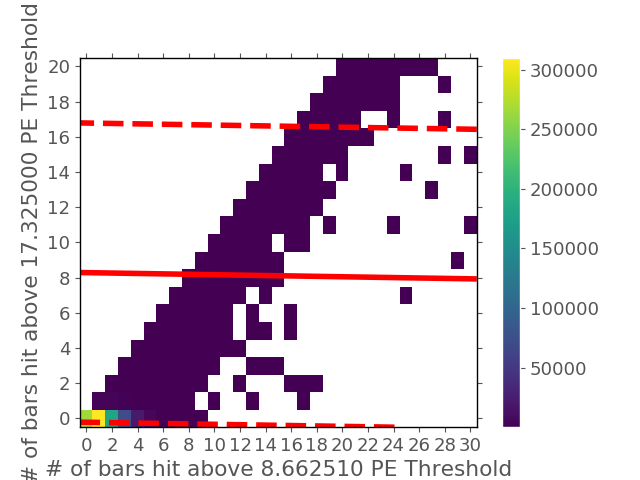
\includegraphics[width=\linewidth]{Chapter5/Figs/Raster/Cosmic8BarNoiseZoomCutSVM.png}
%   \captionsetup{width=.9\linewidth}
%   \caption{}
%   \label{subFig:Cosmic8BarNoiseZoomCutSVM}
% \end{subfigure}
% \caption{Zoomed in version of figure \ref{fig:cosmic8BarSignalNoiseCutSVM} to show how effective the SVM is at removing noise. In (a) the muon data is represented. In (b) the noise data is represented.}
% \label{fig:Cosmic8BarSignalNoiseZoomCutSVM}
% \end{figure}

The correlation between the muon data and trigger cycle 18 can be seen in figure \ref{fig:badCycles}. There is a clear exponential like increase in candidates leading up to trigger cycle 18 and the overflow cycles 17 and 19, this indicates trigger sculpting. By looking at the control data in cycles 20--22 which has no correlation to the trigger a maximum rate of $\sim 2.5 \times 10^5$ is observed in cycle 20. Therefore, all events that have a count rate above cycle 20 are correlated to the trigger and are therefore considered biased as annotated in figure \ref{fig:badCycles}. These cycles cannot be used for cosmic muon tomography due to their severe bias on the left hand side of side A and side B (figure \ref{fig:sideABHitsWithBadCycles}). If these biased events are used the tomography becomes significantly distorted, and by extension so will any shadows. Ideally, figure \ref{fig:sideABHitsWithBadCycles} should show a roughly uniform distribution across both sides. When these events are removed the bias on the left of each side is no longer present as shown in figure \ref{fig:wylfaSideABHits}. This indicates that most of the Wylfa data is not suitable for this approach. But a small portion of the data ($\sim 3 \times 10^6$ events) was unbiased and so could used for tomography. Figures \ref{fig:badCycles} and \ref{fig:sideABHitsWithBadCycles} show the affect trigger sculpting has on the cosmic muon data. The majority of the muon events that get past the trigger have $\theta$ values < 90$^\circ$. Therefore, once side B has had 3 columns removed to match side A both show a statistical increase towards the upper left hand side as a result of these angled ``corner clipping'' muons.

% In addition, some cycles that contain muon data are correlated to the trigger cycle 18. These cycles are considered as ``bad'' for cosmic muon data because they are biased towards the trigger cycles. These bad cycles are shown in figure \ref{fig:badCycles}. Whether a cycle is considered bad depends on whether or not its count rate is above the count rate for cycle 20 in figure \ref{fig:badCycles}. If these bad cycles are added into the data set strange biasing occurs at the side left-hand side of side A and side B as seen in figure \ref{fig:sideABHitsWithBadCycles}. These results are a direct effect of the electronic biasing when taking cosmic muon data in accidental coincidence and are not a result of track fitting. As will be shown in section \ref{sec:SimulationOfCosmics} the tracker seems to have no obvious biasing associated with it. % as shown later in figures \ref{fig:wylfaSideABHits} and \ref{fig:liverpoolSideABHits} the track fitter does not seem to cause any biasing. 

\begin{figure}[!h]
 \centering
 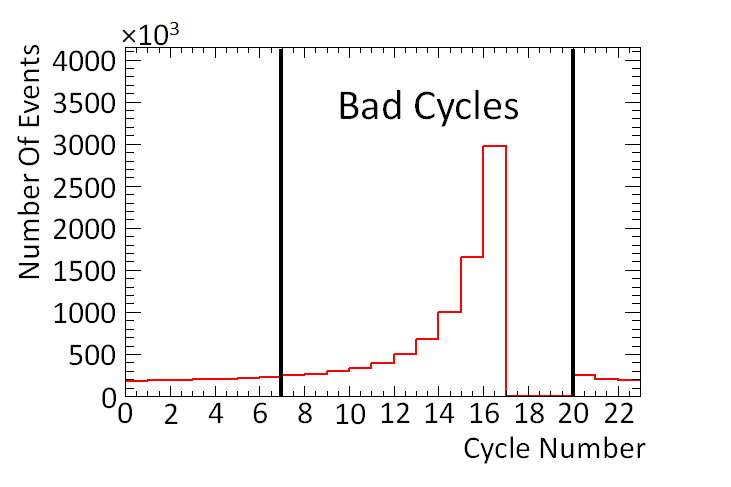
\includegraphics[width=0.7\linewidth]{Chapter6/Figs/Raster/badCyclesRedoMedText.png}
 \captionof{figure}[Timing cycles for the measured cosmic muons at Wylfa.]{Cycles for the measured cosmic muons at Wylfa. The trigger cycles (17, 18, and 19 are already removed). Cycles are considered biased towards the trigger if their count rate exceeds cycle 20's (the control data).} 
 \label{fig:badCycles}
\end{figure}

\begin{figure}[!h]
\centering
\begin{subfigure}{.5\textwidth}
  \centering
  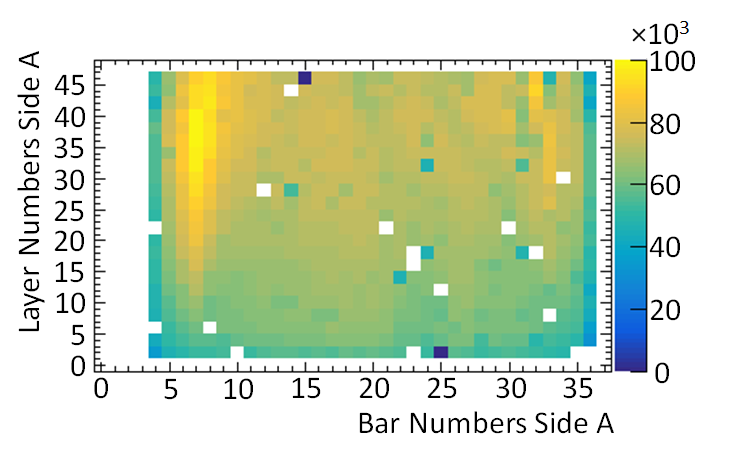
\includegraphics[width=\linewidth]{Chapter6/Figs/Raster/sideAHitsWithBadCyclesMedText.png}
  \captionsetup{width=.9\linewidth}
  \caption{} 
  \label{subFig:sideAHitsWithBadCycles}
\end{subfigure}%
\begin{subfigure}{.5\textwidth}
  \centering
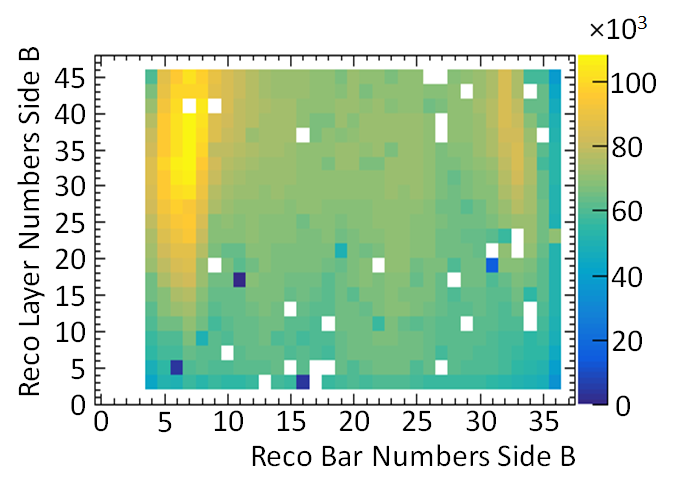
\includegraphics[width=\linewidth]{Chapter6/Figs/Raster/sideBHitsWithBadCyclesMedText.png}
  \captionsetup{width=.9\linewidth}
  \caption{}
  \label{subFig:sideBHitsWithBadCycles}
\end{subfigure}
\caption[Cosmic muon bar hits when biased timing cycles are included.]{Bar hits for cosmic muons at Wylfa when reconstructed with the tracker when biased cycles are included. Side A is shown in (a). Side B is shown in (b). Large streaks are visible on the left-hand sides of both side A and side B.}
\label{fig:sideABHitsWithBadCycles}
\end{figure}

\begin{figure}[!h]
\centering
\begin{subfigure}{.5\textwidth}
  \centering
  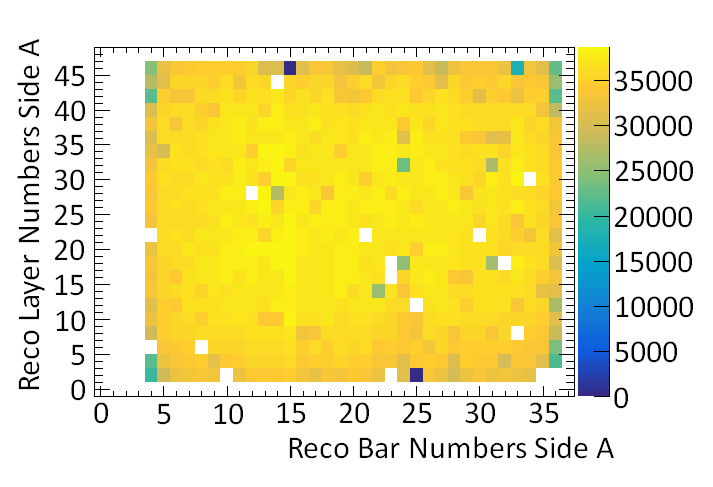
\includegraphics[width=\linewidth]{Chapter6/Figs/Raster/wylfaSideAHitsMedText.png}
  \captionsetup{width=.9\linewidth}
  \caption{}
  \label{subFig:wylfaSideAHits}
\end{subfigure}%
\begin{subfigure}{.5\textwidth}
  \centering
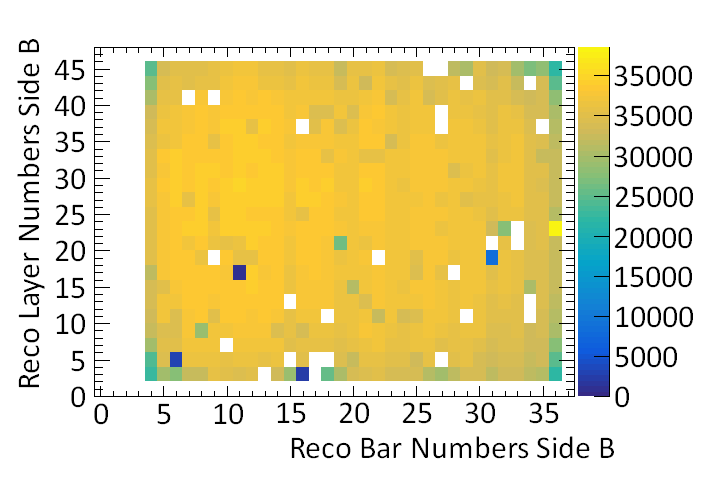
\includegraphics[width=\linewidth]{Chapter6/Figs/Raster/wylfaSideBHitsMedText.png}
  \captionsetup{width=.9\linewidth}
  \caption{}
  \label{subFig:wylfaSideBHits}
\end{subfigure}
\caption[Cosmic muon bar hits when biased timing cycles are excluded.]{Bar hits for sides A and B cosmic muon reconstructed tracks for the accumulated Wylfa data set. The results mostly show a flat profile except for a few dead or almost dead channels, and one noisy channel on side B. This suggests the tracker exhibits minimal bias. Side A is shown in (a). Side B is Shown in (b)}
\label{fig:wylfaSideABHits}
\end{figure}

%white space 
%\vspace{960pt}

\section{Reactor Shadow: Methodology} \label{sec:ReactorShadowMethodology}
In order to validate any shadows present at the reactor site the detector position relative to any buildings that block cosmic muons must be determined. Figure \ref{subFig:DetectorPositionTopDown} already shows the detector position as observed by Google Earth. In figure \ref{subFig:wylfaTraceStep1}, the buildings have had simple shapes overlaid with a corresponding key to highlight the buildings of interest. In figure \ref{subFig:wylfaTraceStep2} these shapes are then offset to account for the building heights relative to the detector and the angle of the aerial photograph. The most obvious reference points visible in figure \ref{subFig:wylfaTraceStep1} being the top left of the main reactor building and top left of the turbine hall denoted with a magenta cross. Finally, the connecting lines and the background aerial photo from figure \ref{subFig:wylfaTraceStep2} are removed to produce figure \ref{subFig:wylfaTraceStep4}, producing the final clean trace. In figures \ref{subFig:wylfaTraceStep1}  -- \ref{subFig:wylfaTraceStep4} the size of the reactor core area the size and shape of the reactor core has been estimated as a cylinder of $\sim$ 25\,m diameter \cite{rMillsReactorSize} including both the reactor core and reactor core shielding. The height of the reactor core was assumed to be $\sim$ 25\,m as well, but as figure \ref{fig:wylfaReactorRoughStructure} shows the shielding does curve upwards and so may appear taller than this. These width and height assumptions are later corroborated with measurements from the Wylfa data set. 

\begin{figure}[!h]
\centering
\begin{subfigure}{.5\textwidth}
  \centering
  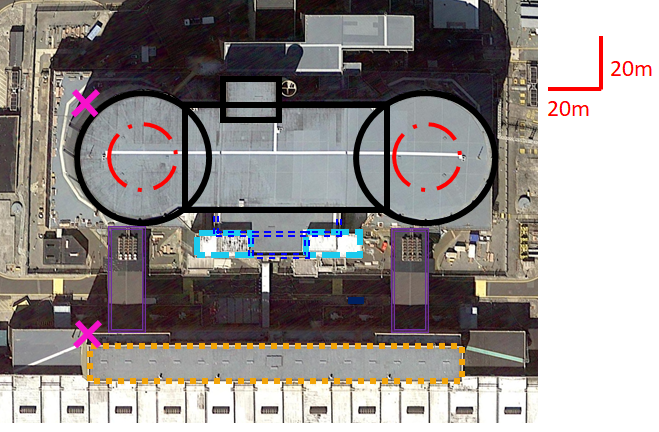
\includegraphics[width=\linewidth]{Chapter6/Figs/wylfaTraceStep1NoLeg.png}
  \captionsetup{width=.9\linewidth}
  \caption{}
  \label{subFig:wylfaTraceStep1}
\end{subfigure}%
\begin{subfigure}{.5\textwidth}
  \centering
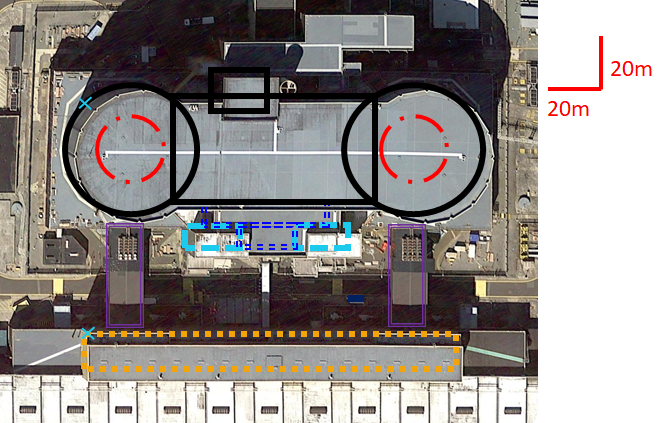
\includegraphics[width=\linewidth]{Chapter6/Figs/wylfaTraceStep2NoLeg.png}
  \captionsetup{width=.9\linewidth}
  \caption{}
  \label{subFig:wylfaTraceStep2}
\end{subfigure}
\begin{subfigure}{1.0\textwidth}
  \centering
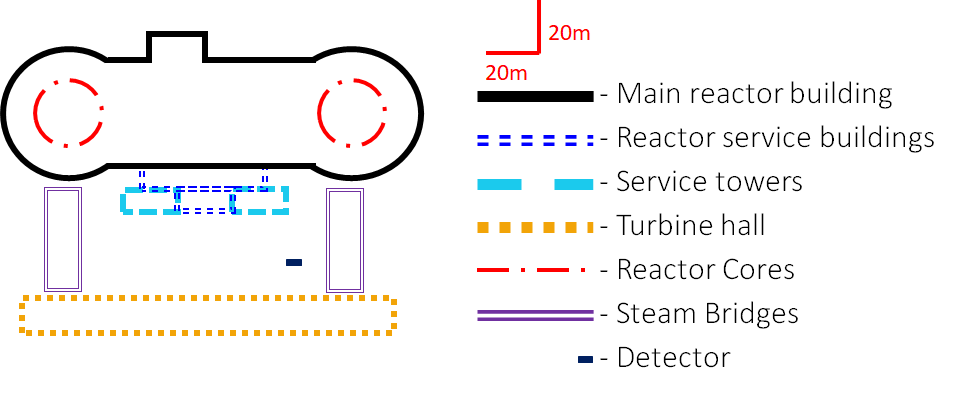
\includegraphics[width=\linewidth]{Chapter5/Figs/wylfaRasterNew/wylfaTraceStep4.png}
  \captionsetup{width=.9\linewidth}
  \caption{}
  \label{subFig:wylfaTraceStep4}
\end{subfigure}
\caption[Detector position with buildings of interest.]{Detector position with buildings of interest. (a) is a basic trace on top of figure \ref{subFig:DetectorPositionTopDown}. Basic shapes are overlaid on top of the buildings at Wylfa. In (b) the trace is adjusted to take the overhead camera's position into account by taking the base of the buildings and moving the trace towards the base of the buildings. The magenta $\times$s show the reference points used to account for the camera's position. In (c) the overlapping lines and aerial photography from Google Earth removed to produce the final trace with a corresponding key.}
\label{fig:wylfaTraceSteps1-4}
\end{figure}

% \begin{figure}[!h]
%  \centering
%  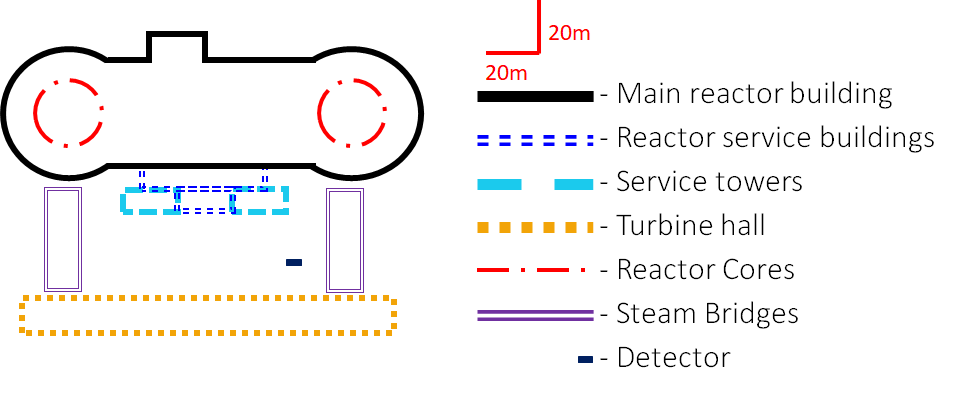
\includegraphics[width=\linewidth]{Chapter5/Figs/wylfaRasterNew/wylfaTraceStep4.png}
%  \captionof{figure}{}
%  \label{fig:wylfaTraceStep4}
% \end{figure}

Now that figure \ref{subFig:wylfaTraceStep4} has been produced and the features of interest have been identified, the cosmic muon data needs to be analysed. The logic for the track reconstruction is outlined in section \ref{sec:SimulationOfCosmics}, using that tracker the Wylfa data can be fitted. An example is shown in figure \ref{fig:3000ExampleEventWithKey}. In figure \ref{fig:3000ExampleEventWithKey} there are many noise hits that can potentially cause the track reconstruction to fail. The tracker has been custom-built around both measured and simulated data to prevent any minimisation issues. There are also three columns of uninstrumented channels on side A which figure \ref{fig:3000ExampleEventWithKey} shows in grey. These uninstrumented channels inform the fiducial boundaries as well, and in figure \ref{fig:3000ExampleEventWithKey} the excluded channels are shown in light blue. The number of columns on side A and side B must be the same otherwise any shadow that the detector will analyse will become distorted in one direction more than the other. Also in figure \ref{fig:3000ExampleEventWithKey} a number of dead channels that also have to be carefully considered when assessing tracker performance. By looking at the tracker reconstructed hits on aggregate in figure \ref{fig:wylfaSideABHits} there does not appear to be any bias in the Wylfa data set. In figure \ref{fig:wylfaSideABHits} there are dead channels and inefficient channels that do not seem to impact the channels surrounding them suggesting the tracker is successfully reconstructing the distribution. The only issue is a single noisy channel in \ref{subFig:wylfaSideBHits} but as the areas around the channel have event rates comparable to their neighbours meaning it is reasonable to assume this is an issue with the channel rather than the reconstruction. 

\begin{figure}[!h]
 \centering
 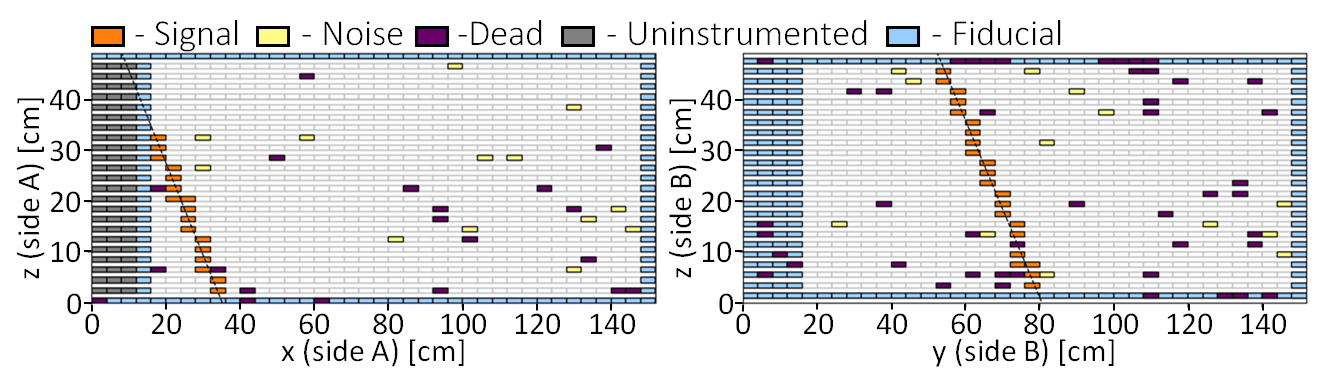
\includegraphics[width=\linewidth]{Chapter6/Figs/Raster/newExampleEventWylfaMedText.png}
 \captionof{figure}[An example event from the Wylfa data set.]{An example event from the Wylfa data set with a corresponding key showing how the colour coding relates to the channels. The solid line represents the fit.} 
 \label{fig:3000ExampleEventWithKey}
\end{figure}

Once the tracker's potential bias has been addressed, the $\phi$ and $\theta$ values can be analysed. Due to the high energy and highly penetrating nature of cosmic muons \cite{Olive_2014} the reactor buildings may not be dense enough to stop all incoming cosmic muons and deflection is a likely possibility. As a result, the shadows can only be seen with a sufficiently high number of events. Due to limitations previously mentioned, there are $\sim 3 \times 10^6$ cosmic muons in the Wylfa data set that are usable. According to the CRY library, \cite{ieee_cry_2007} 162000 muons and 174000 anti-muons are produced in 2820\,s for 1\,m$^2$. VIDARR's top surface areas are both 1.52\,m $\times$ 1.52\,m = 2.31\,m$^2$ resulting in $\sim$ 275 muon per second. Therefore, a data set of 3 $\times$ 10$^6$ cosmic muon events corresponds to $\sim$ 3 hours of live time. With a rate of 275 muons per second the maximum time the reconstruction should be allowed to take is 3.6\,ms for online track reconstruction which figure \ref{subFig:wylfaTrackerTime} shows is the case for almost all events. Figure \ref{fig:wylfaTrackerTimeAndLog} shows that only a very small fraction of events are not successfully reconstructed within the time limit of 3.6\,ms so a time selection criteria will be required for online track fitting. Whilst online track reconstruction was not required, it is useful to know that the same reconstruction code can be applied for both online calibration and full cosmic muon tomography by only adding a processing time limit. 

\begin{figure}[!h]
\centering
\begin{subfigure}{.5\textwidth}
  \centering
  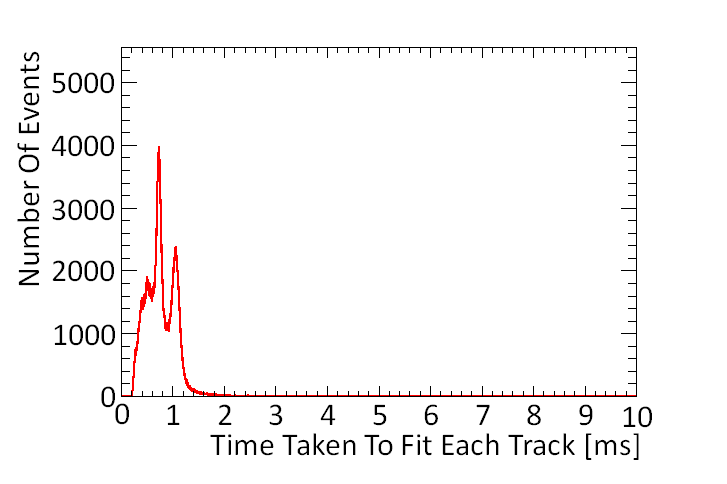
\includegraphics[width=\linewidth]{Chapter6/Figs/Raster/wylfaTrackerTimeMedText.png}
  \captionsetup{width=.9\linewidth}
  \caption{}
  \label{subFig:wylfaTrackerTime}
\end{subfigure}%
\begin{subfigure}{.5\textwidth}
  \centering
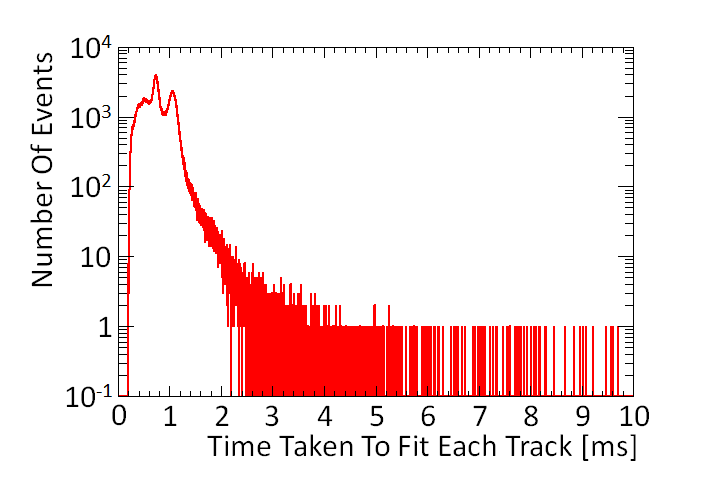
\includegraphics[width=\linewidth]{Chapter6/Figs/Raster/wylfaTrackerTimeLogMedText.png}
  \captionsetup{width=.9\linewidth}
  \caption{}
  \label{subFig:wylfaTrackerTimeLog}
\end{subfigure}
\caption[The time taken for each fit for the Wylfa data set.]{(a) The time taken for each fit for the Wylfa data set. Assuming a rate of $\sim$ 275 cosmic muons per second then the maximum time allowed would be 3.6\,ms. Almost all cosmic candidate events fit within this time. In (b) the y axis taken as a log, some events exceed 3.6\,ms to fit so a maximum time selection criterion is needed for those events.}
\label{fig:wylfaTrackerTimeAndLog}
\end{figure}

The reconstructed $\phi$ and $\theta$ distribution from the Wylfa data set can be seen in figure \ref{fig:pVsTWylfaReversed} but the shadows are not as differentiated as one would have expected from such large and dense buildings. In figure \ref{fig:pVsTWylfaReversed} the bin migration is so significant even though the shadows extend up to 60$^o$ in $\theta$, they are effectively masked. The bin migration does become less pronounced as $\theta$ decreases (see section \ref{sec:SimulationOfCosmics}). However, this poses a problem as the statistics also decrease with $\theta$ as seen in figure \ref{fig:pVsTWylfaReversed}. So by taking the 2D $\phi$ projection of figure \ref{fig:pVsTWylfaReversed} from 0$^\circ$ -- 37.5$^\circ$ in $\theta$, it is possible to ignore most of the bin migration whilst also having suitable statistics to observe the widths of the turbine hall and reactor buildings (figure \ref{fig:LinearHist_theta_0-37.5_Deg}). Figure \ref{fig:LinearHist_theta_0-37.5_Deg} is then shown via a polar histogram and overlaid on top of the Wylfa trace (figure \ref{subFig:wylfaTraceStep4}) producing figure \ref{fig:wylfaCircular0-37.5Deg_Overlay}. 

\begin{figure}[!h]
\centering
\begin{minipage}{.45\textwidth}
  \centering
  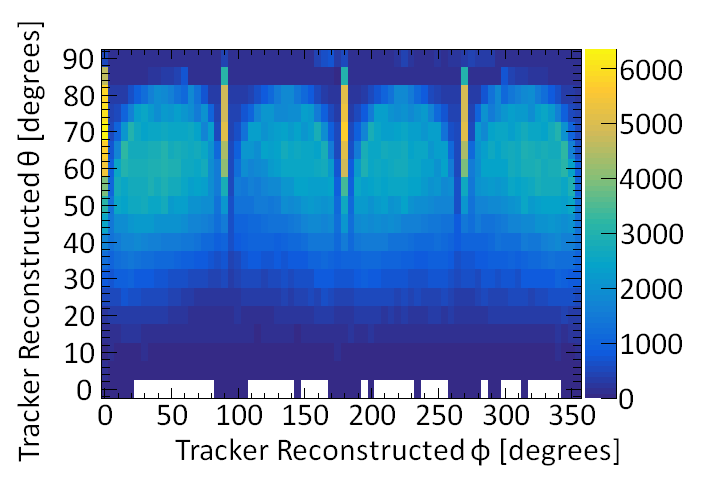
\includegraphics[width=\linewidth]{Chapter6/Figs/Raster/pVsTWylfaReversedMedText.png}
  \captionof{figure}[Cosmic muon distribution from the deployment at the Wylfa reactor site.]{The cosmic muon distribution from the deployment at the Wylfa reactor site, the shadows extend from $\theta$ = 0$^\circ$ -- $\theta$ = 60$^\circ$. But bin migration causes significant warping.}
  \label{fig:pVsTWylfaReversed}
  \vspace{1.434cm} %1 line = 0.478cm % 2 lines = 0.956cm % 3 lines= 1.434cm % 4 lines = 1.912cm % 5 lines = 2.39cm
\end{minipage}%
\qquad
\begin{minipage}{.45\textwidth}
  \centering
  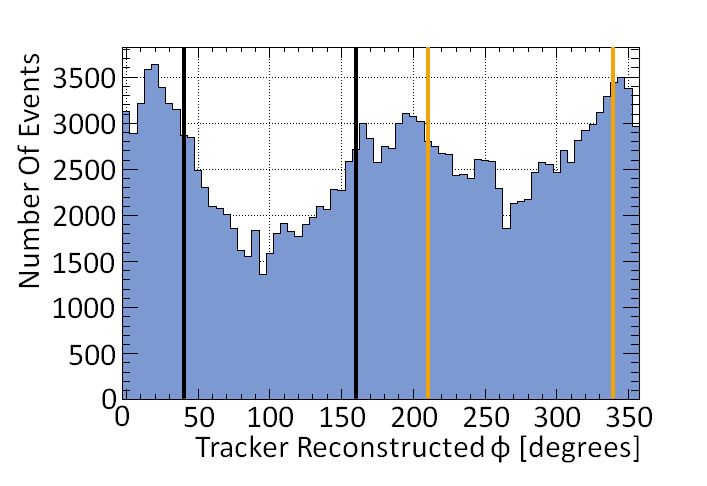
\includegraphics[width=\linewidth]{Chapter6/Figs/Raster/LinearHist_theta_0-37.5_DegMedText.png}
  \captionof{figure}[Linear histogram showing a 2d projection of $\phi$.]{Linear histogram showing a 2d projection of figure \ref{fig:pVsTWylfaReversed} from $\theta$ = 0$^\circ$ -- $\theta$ = 37.5$^\circ$ this range was chosen to avoid as much bin migration as possible whilst having as high statistics as possible. The main reactor shadow is highlighted by black lines the turbine hall is highlighted by orange lines.}
  \label{fig:LinearHist_theta_0-37.5_Deg}
\end{minipage}
\end{figure}

 \begin{figure}[!h]
 \centering
 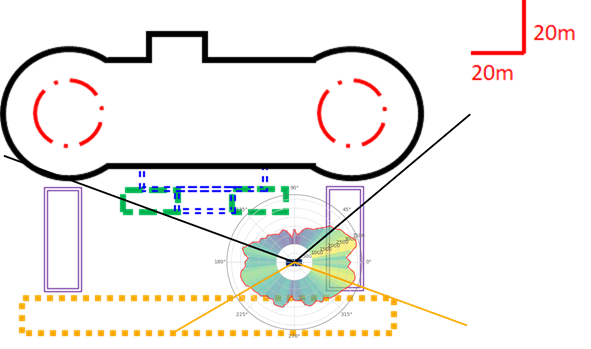
\includegraphics[width=0.7\linewidth]{Chapter5/Figs/wylfaRasterNew/wylfaCircular0-37.5Deg_Overlay.png}
 \captionof{figure}[Top down trace of the Wylfa reactor site.]{Top down trace of the Wylfa reactor site (Figure \ref{subFig:wylfaTraceStep4}) overlaid with the circular histogram from figure \ref{fig:LinearHist_theta_0-37.5_Deg} to show how the borders line up with the trace.} 
 \label{fig:wylfaCircular0-37.5Deg_Overlay}
\end{figure}

Figure \ref{fig:wylfaCircular0-37.5Deg_Overlay} also shows the limitation of this method. Whilst there are several buildings that block incident cosmic muons, only the largest building (the main reactor building) and the closest building (the turbine hall) are visible. In addition, the far edge of the turbine hall is not clear in figure \ref{fig:wylfaCircular0-37.5Deg_Overlay}, even though it should be. This is due to the turbine hall being composed of corrugated steel, thus blocking fewer cosmic muons. The results from figures \ref{fig:pVsTWylfaReversed} -- \ref{fig:wylfaCircular0-37.5Deg_Overlay} match closely the expected shape as figure \ref{fig:sideBySideComparisonTopDownCirc} shows. 

%  \begin{figure}[!h]
%  \centering
%  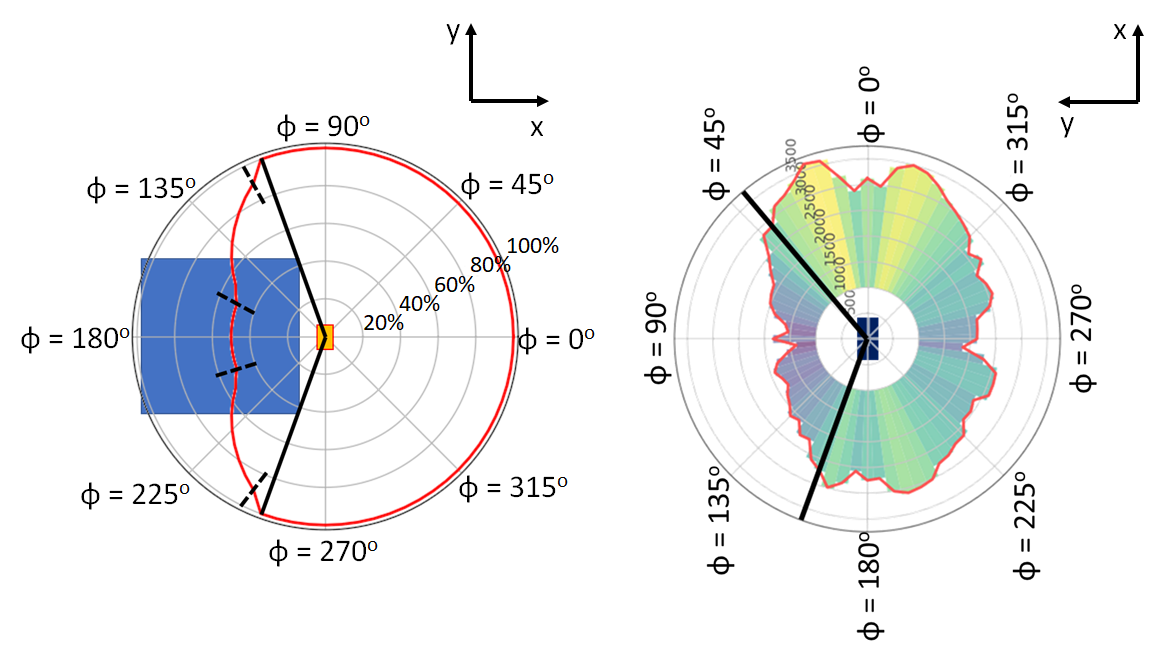
\includegraphics[width=\linewidth]{Chapter6/Figs/Raster/sideBySideComparisonTopDownCircMedText.png}
%  \captionof{figure}{How the polar Wylfa histogram compares to a basic expectation the large tails are visible in both producing a similar shape.}
%  \label{fig:sideBySideComparisonTopDownCirc}
% \end{figure}

\begin{figure}[!h]
\centering
\begin{subfigure}{.5\textwidth}
  \centering
  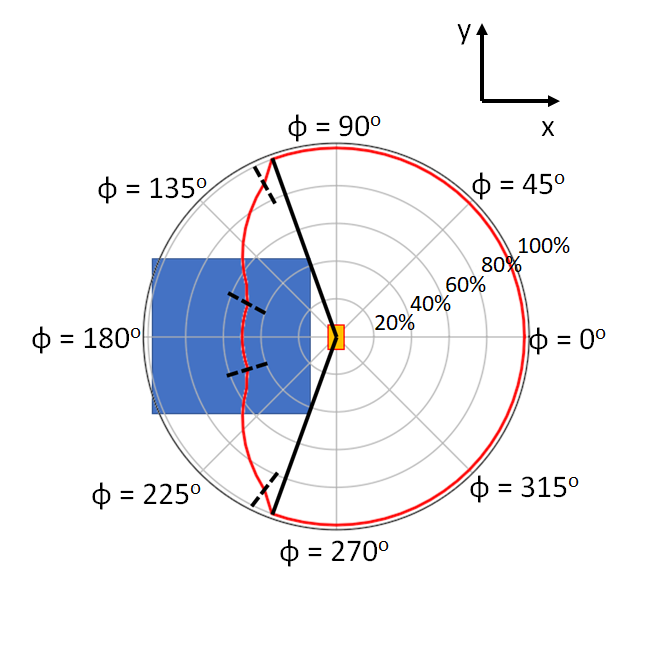
\includegraphics[width=\linewidth]{Chapter6/Figs/Raster/expectedCubeAttenuation.png}
  \captionsetup{width=.9\linewidth}
  \caption{}
  \label{subFig:expectedCubeAttenuation}
\end{subfigure}%
\begin{subfigure}{.5\textwidth}
  \centering
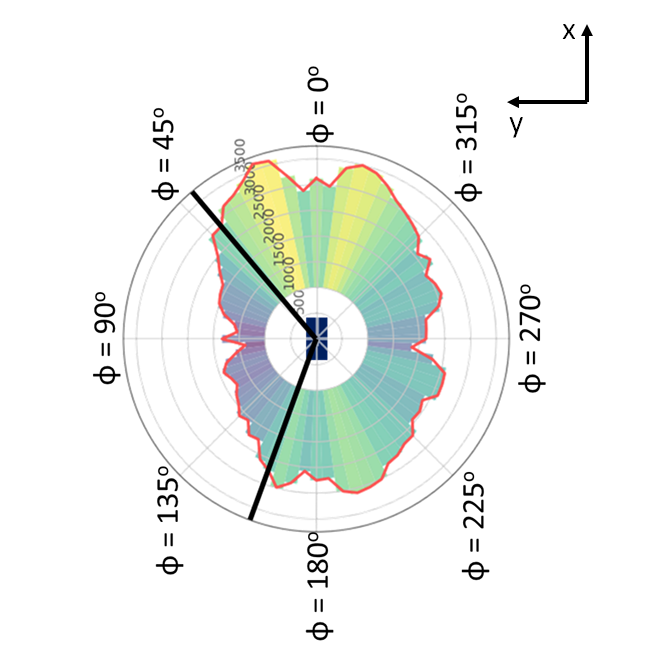
\includegraphics[width=\linewidth]{Chapter6/Figs/Raster/measuredWylfaAttenuation.png}
  \captionsetup{width=.9\linewidth}
  \caption{}
  \label{subFig:measuredWylfaAttenuation}
\end{subfigure}
\caption[Polar histogram comparison of a simulated cuboid block of material.]{Polar histogram comparison of a simulated cuboid block of material (a) to the Wylfa data set (b). This shows that the dense cuboid approximates the dens reactor building and its effect on the incident muon distribution.}
\label{fig:sideBySideComparisonTopDownCirc}
\end{figure}

A way to solve the issue of bin migration was highlighted in section \ref{sec:geologicalTomography} which is to use the transmission method the MU-RAY collaboration used \cite{Ambrosino_2014}. The transmission method uses the ratio of the data with the cosmic muon occlusion and a control data set which has minimal to no muon occlusion. In order for this to work, another data set that reconstructs the whole hemisphere in $\phi$ and $\theta$ is required. It might be possible to use simulated cosmic data to achieve this result however the atmospheric scattering is not taken into account properly (as will be shown in section \ref{sec:usingSimulatedDataAsControlData}). The best approach would be to use control data in the same location after the demolition of the Wylfa buildings, but as that will take decades, this is infeasible. Instead, measured data was taken at Liverpool from 2016 -- 2018 which produced figure \ref{fig:pVsTLiverpoolReversed}. There are some shadows in the Liverpool data specifically from the accelerator hall at low angles of $\theta$ from 0$^\circ$ -- 17.5$^\circ$ which is shown in figure \ref{fig:liverpoolShadows}. However, once those ranges are removed from the data set it serves as a useful control data set as there is minimal cosmic muon sky occlusion. When checking for any potential bias in the Liverpool data set, none is visible for either side as shown in figure \ref{fig:liverpoolSideABHits}. 

\begin{figure}[!h]
\centering
\begin{minipage}{.45\textwidth}
  \centering
  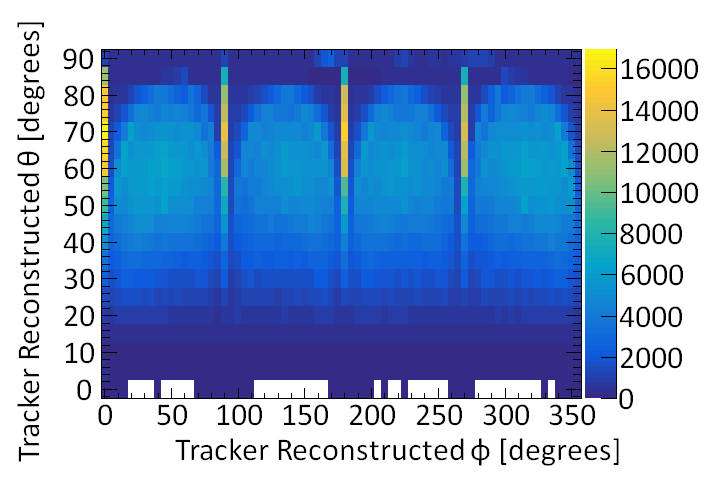
\includegraphics[width=\linewidth]{Chapter6/Figs/Raster/pVsTLiverpoolReversedMedText.png}
  \captionof{figure}[The cosmic muon distribution from the deployment at Liverpool.]{The cosmic muon distribution from the deployment at Liverpool. There are some faint shadows below 17.5$^\circ$ but otherwise the data has no major cosmic muon sky occlusion.} 
  \label{fig:pVsTLiverpoolReversed}
\end{minipage}%
\qquad
\begin{minipage}{.45\textwidth}
  \centering
  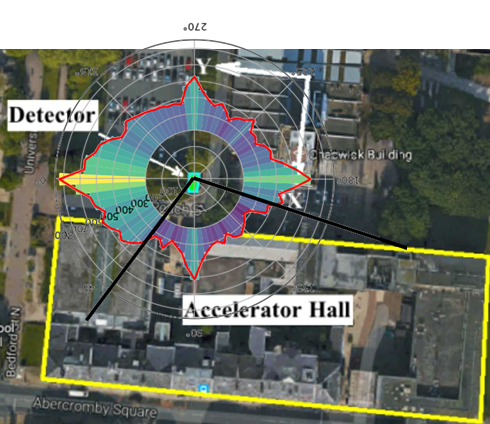
\includegraphics[width=\linewidth]{Chapter5/Figs/Raster/liverpoolShadows.png}
  \captionof{figure}[The shadows in the Liverpool data below $\theta$ =  17.5$^\circ$.]{The shadows in the Liverpool data below $\theta$ =  17.5$^\circ$. The accelerator hall causes significant cosmic muon occlusion but only below 17.5$^\circ$.}
  \label{fig:liverpoolShadows}
  \vspace{1.248cm} %1 line = 0.478cm % 2 lines = 0.956cm % 3 lines= 1.434cm % 4 lines = 1.912cm % 5 lines = 2.39cm
\end{minipage}
\end{figure}

\begin{figure}[!h]
\centering
\begin{subfigure}{.5\textwidth}
  \centering
  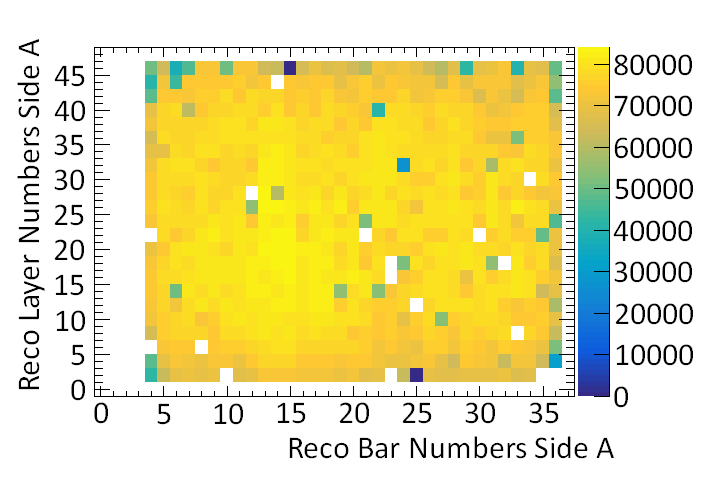
\includegraphics[width=\linewidth]{Chapter6/Figs/Raster/liverpoolSideAHitsMedText.png}
  \captionsetup{width=.9\linewidth}
  \caption{}
  \label{subFig:liverpoolSideAHits}
\end{subfigure}%
\begin{subfigure}{.5\textwidth}
  \centering
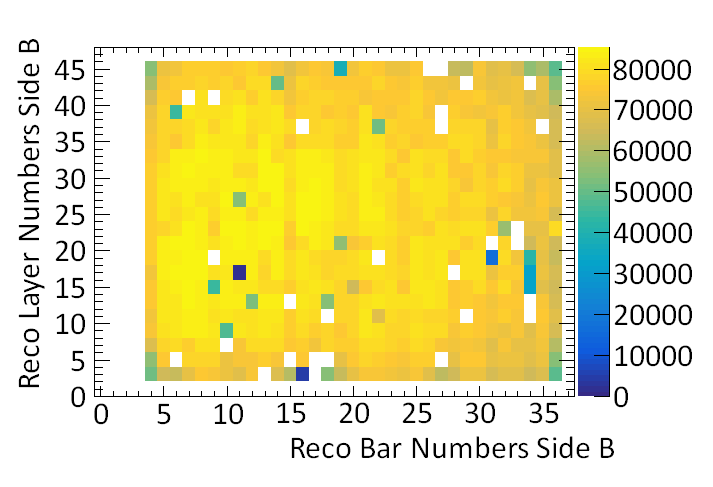
\includegraphics[width=\linewidth]{Chapter6/Figs/Raster/liverpoolSideBHitsMedText.png}
  \captionsetup{width=.9\linewidth}
  \caption{}
  \label{subFig:liverpoolSideBHits}
\end{subfigure}
\caption[Bar hits for sides A and B show the cosmic muon reconstructed tracks for the Liverpool data set.]{Bar hits for sides A and B show the cosmic muon reconstructed tracks for the Liverpool data set. The results are mostly flat except for a few dead or almost dead channels. Suggesting the reconstruction exhibits no or minimal bias. Side A is shown in (a). Side B is shown in (b).}
\label{fig:liverpoolSideABHits}
\end{figure}

When normalising the Liverpool data set (figure \ref{fig:pVsTLiverpoolReversed}) to the Wylfa data set (figure \ref{fig:pVsTWylfaReversed}) then dividing the Wylfa data by the Liverpool data and removing the values below 17.5$^\circ$ in $\theta$ (thus making the Liverpool data suitable for control purposes) a map of the shadows caused by the Wylfa site buildings with minimal detector effects is produced (figure \ref{fig:measuredTrackerReconNoLines}). The shadows are now clearly visible in both $\phi$ and $\theta$ with the main reactor buildings centring around 90$^\circ$ in $\phi$ and the turbine hall centring around 270$^\circ$ in $\phi$. There are several interesting features seen in figure \ref{fig:measuredTrackerReconNoLines} where the top of the turbine hall seen between $\sim$ 240$^\circ$ -- 330$^\circ$ in $\phi$ is not well resolved. This is because the turbine hall is made from corrugated steel and so blocks fewer cosmic muons. Therefore, a significant portion of the building has to be traversed before the top is visible. But the area from 0$^\circ$ -- 180$^\circ$ in $\phi$ is of particular interest as this area contains the main reactor building and corresponding service buildings. As multiple buildings block the path of incident cosmic muons between the detector and reactor building the shadow patterns are much more complex than one would naively expect. In addition, there appears to be an area of high density between 60$^\circ$ -- 80$^\circ$ in $\phi$, 20$^\circ$ -- 25$^\circ$ in $\theta$ which could be the reactor core. In order to determine which components of the shadow are caused by which buildings a simulation is required where each reactor building can be simulated separately.

\begin{figure}[!h]
 \centering
 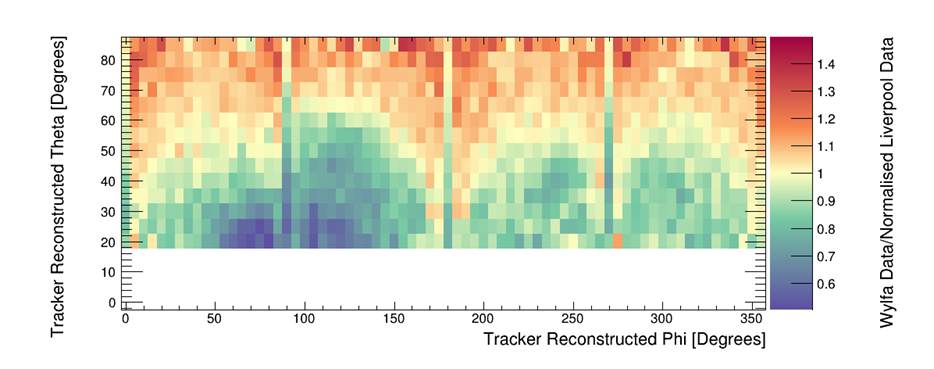
\includegraphics[width=\linewidth]{Chapter5/Figs/wylfaRasterNew/measuredTrackerReconNoLines.png}
 \captionof{figure}[The measured building shadows taking the ratio of the Wylfa data set.]{The measured building shadows taking the ratio of the Wylfa data set (figure \ref{fig:pVsTWylfaReversed}) and the Liverpool data set (figure \ref{fig:pVsTLiverpoolReversed}). The Liverpool data acts as a control data set, assuming minimal shadows are present in the Liverpool data above 17.5$^\circ$ in $\theta$.} 
 \label{fig:measuredTrackerReconNoLines}
\end{figure}

The simulation previously mentioned in chapters \ref{chp:GEANT4Simulation} and \ref{chp:DataAnalysisTechniques} has the detector as the centre of the simulation world in the $x$ and $y$ and put the detector on the ground at  $z = 0 $. Hence all of the reactor buildings need to be positioned relative to the detector and also placed at $z = 0$ (with the exception of the elevated steam bridges). The Wylfa trace seen in figure \ref{subFig:wylfaTraceStep4} can be approximated by placing simple shapes on top of the trace as seen in figure \ref{fig:simulatedPositions}. Figure \ref{fig:simulatedPositions} also clearly labels each major building box, the positions for each box and in $x$ and $y$ and the widths and depths are approximated based on this figure/trace and are given in table \ref{tab:simulatedBuildingPositions} (and appendix \ref{appenC:ReactorBuildingEdges}). Finally, the heights have to be approximated: this is difficult due to the distortion the top portions of buildings are subject to as part of projecting a comic hemisphere distribution onto a cuboid. In addition, distance from the detector, height, building shape and construction are all combined into a single measurement. This is the main reason the building widths are estimated from aerial photography (Google Earth) rather than from on-site measurements. Sadly, no information pertaining to heights has been preserved. It is tempting to use the measurements of $\theta$ to produce reconstructions of the heights via equation \ref{equ:tanHeightEquation} with the lengths provided by Google Earth. But this approach makes two key assumptions: 1. perfectly solid uniform buildings 2. minimal scattering of cosmic muons. Assumption 1 is known to be inaccurate from figure \ref{fig:wylfaReactorRoughStructure}. Assumption 2 is naive considering the high Z values and densities of the materials used in the construction of the reactor buildings. As a result, it is best to use the estimates provided by equation \ref{equ:tanHeightEquation} and then iterate over different heights in the simulation to match the shadow shapes seen in figure \ref{fig:measuredTrackerReconNoLines}. The approximate heights and $z$ positions are also shown in table \ref{tab:simulatedBuildingPositions}. Ideally, the heights in the simulation would be resolved by going on-site and taking detailed measurements. Due to the decommissioning currently taking place at the Wylfa site, this is not possible. Appendix \ref{appenC:ReactorBuildingEdges} contains the remaining building boxes simulated, the boxes which are used to emulate the distinctive ``dog bone'' shape of the main reactor building at Wylfa.

\begin{equation}
H = \frac{L}{\tan{\theta}}
\label{equ:tanHeightEquation}
\end{equation}

 \begin{figure}[!h]
 \centering
 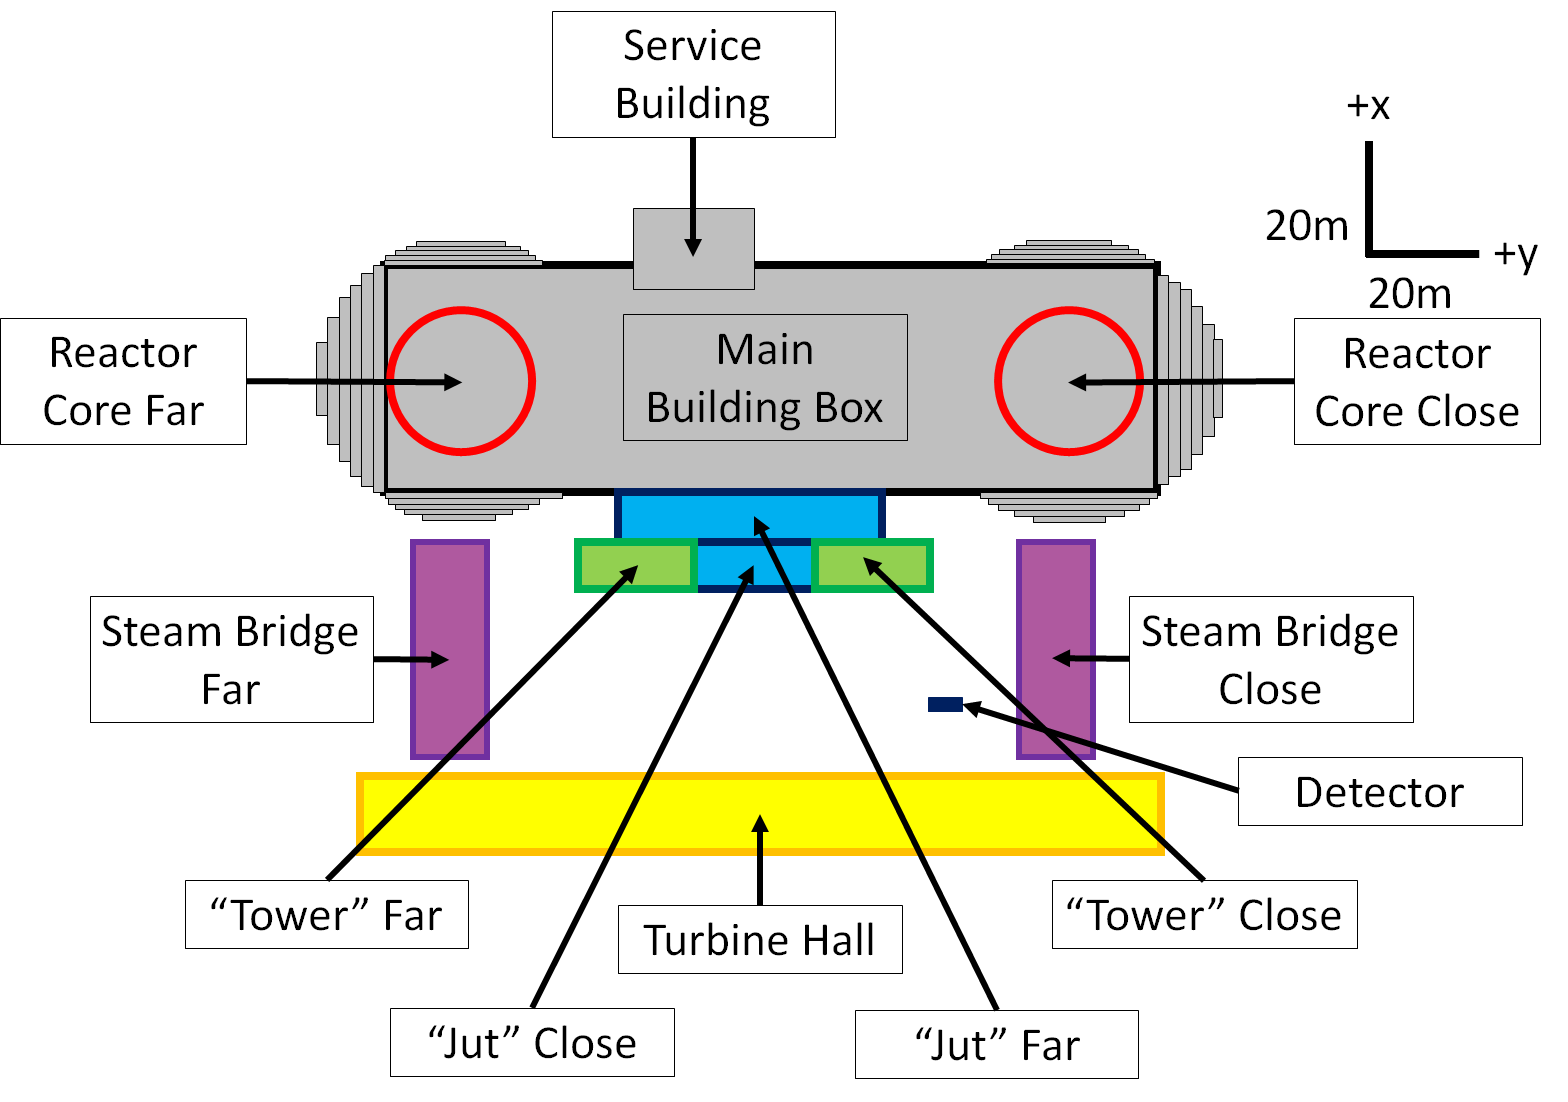
\includegraphics[width=0.7\linewidth]{Chapter6/Figs/Raster/simulatedAnotatedBuildings.png}
 \captionof{figure}[Wylfa track with boxes overlaid on top of buildings of interest.]{The Wylfa trace (figure \ref{subFig:wylfaTraceStep4}) with boxes overlaid to recreate the buildings of interest and circles to represent the reactor cores. The scale from the Wylfa trace (top right) is used to determine the buildings' the correct positions and dimensions in GEANT4, a full list of which can be seen in table \ref{tab:simulatedBuildingPositions}. The edges for the ``dog bone'' shape are shown in appendix \ref{appenC:ReactorBuildingEdges}.} 
 \label{fig:simulatedPositions}
\end{figure}

% \begin{figure}[!h]
%  \centering
%  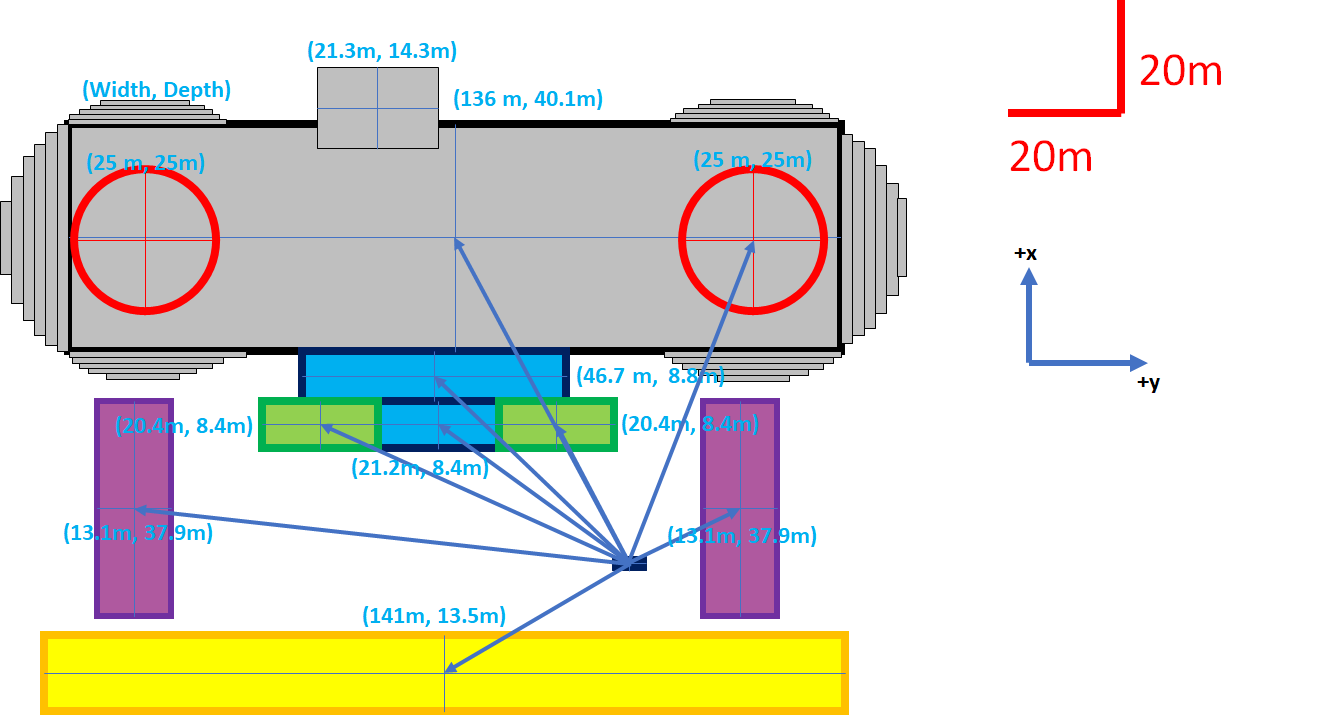
\includegraphics[width=0.8\linewidth]{Chapter5/Figs/wylfaRasterNew/simulatedWidthsDepths.png}
%  \captionof{figure}{Widths and depths from the Wylfa trace (figure \ref{fig:wylfaTraceStep4}) with their widths and depths labelled these were then put into GEANT4.} 
%  \label{fig:simulatedWidthsDepths}
% \end{figure}

% \begin{figure}[!h]
%  \centering
%  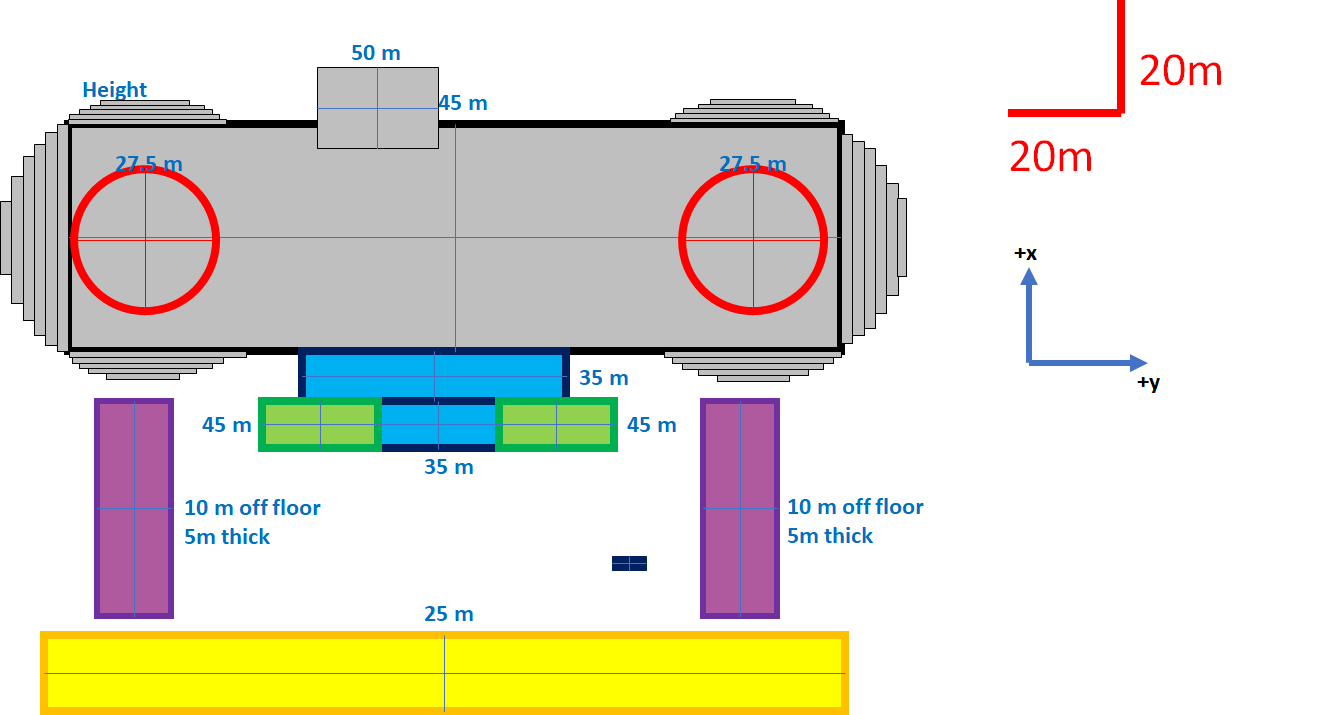
\includegraphics[width=0.8\linewidth]{Chapter5/Figs/wylfaRasterNew/simulatedHeights.png}
%  \captionof{figure}{Heights estimated from the measured data at Wylfa (figure \ref{fig:pVsTWylfaReversed}) these were then put into GEANT4.} 
%  \label{fig:simulatedHeights}
% \end{figure}

\begin{table*}[!h]
\centering
\begin{tabular}{lrrrrrrr}  
\toprule
\multicolumn{1}{c}{} & \multicolumn{3}{c}{Position} & \multicolumn{3}{c}{Dimension} \\
\cmidrule(r){2-4}
\cmidrule(r){5-7}
Building               & X\,[m] & Y\,[m] & Z\,[m] & Width\,[m] & Depth\,[m] & Height\,[m]\\
\midrule
Reactor Core Close     & 57.1   &  22.2  & 0.0     & 25.0       & 25.0       & 27.5\\
Reactor Core Far       & 57.1   & -85.3  & 0.0     & 25.0       & 25.0       & 27.5\\
Main Building Box      & 57.5   & -30.8  & 0.0     & 40.1       & 136.0      & 45.0\\
Sub Building Box       & 80.5   & -44.6  & 0.0     & 14.3       & 21.3       & 50.0\\
Service Building Close & 24.4   & -33.6  & 0.0     & 8.4        & 21.2       & 35.0\\
Service Building Far   & 33.0   & -34.4  & 0.0     & 8.8        & 46.7       & 35.0\\
Service Tower Close    & 24.4   & -12.8  & 0.0     & 8.4        & 20.4       & 45.0\\
Service Tower Far      & 24.4   & -54.5  & 0.0     & 8.4        & 20.4       & 45.0\\
Steam Bridge Close     & 9.73   &  19.7  & 10.0    & 37.9       & 13.1       & 5.0\\
Steam Bridge Far       & 9.73   & -87.7  & 10.0    & 37.9       & 13.1       & 5.0\\
Turbine Hall           & -19.2  & -32.7  & 0.0     & 13.5       & 141.0      & 25.0\\
\bottomrule  
\end{tabular}
\caption{The positions and dimensions for each of the simulated buildings in GEANT4 outlined in figure \ref{fig:simulatedPositions}, relative to the detector which is the origin.}
\label{tab:simulatedBuildingPositions}
\end{table*}

Figure \ref{fig:WylfaSimGeom_SideOn_TopDown} shows the simulated geometry in  GEANT4. The side-on view can be seen in figure \ref{subFig:WylfaSimGeomSideOn} which has the heights annotated, and the top-down view can be seen in figure \ref{subFig:WylfaSimGeomTopDown} which looks similar to figure \ref{fig:simulatedPositions}. Once these dimensions have been approximated, it is possible to simulate detector surroundings both with and without buildings. This is done in figure \ref{fig:thetaVsPhiSimulatedWithReactor_0-100}, using a data driven realistic $\theta$ distribution from Liverpool, and it shows how the bin migration effects compare to the shadows. In the simulation the buildings were simulated as 100\,\% concrete, so they block as many cosmic muons as possible to give accurate building outlines. Then, as with the shadows at Wylfa (figure \ref{fig:measuredTrackerReconNoLines}), the ratio of the data with and without buildings is taken, producing the simulated shadows with minimal detector effects (figure \ref{fig:simulatedTrackerReconNoLines}). 

\begin{figure}[!h]
\centering
\begin{subfigure}{.5\textwidth}
  \centering
  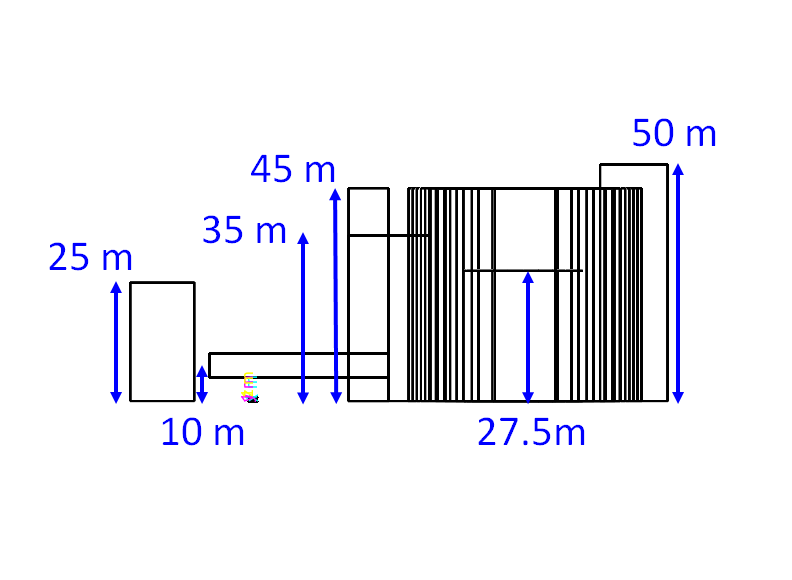
\includegraphics[width=0.9\linewidth]{Chapter5/Figs/wylfaRasterNew/WylfaSimGeomSideOn.png}
  \captionsetup{width=.9\linewidth}
  \caption{}
  \label{subFig:WylfaSimGeomSideOn}
\end{subfigure}%
\begin{subfigure}{.5\textwidth}
  \centering
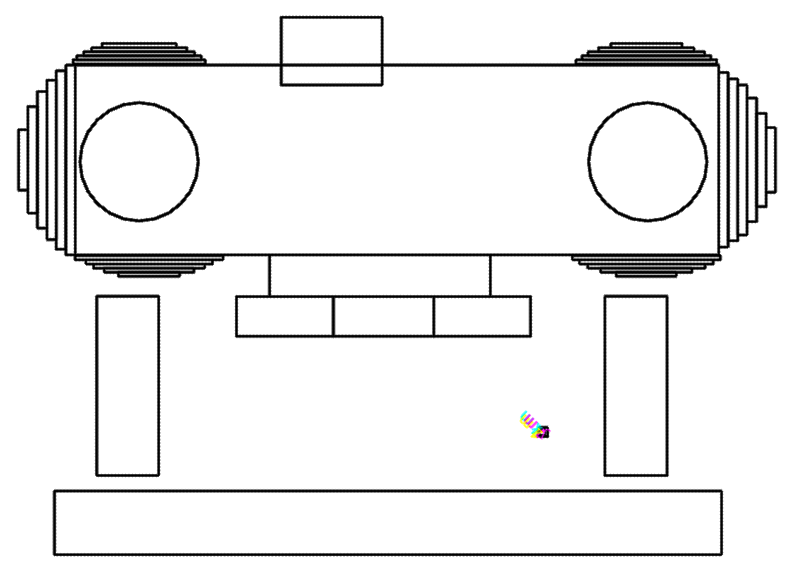
\includegraphics[width=0.9\linewidth]{Chapter5/Figs/wylfaRasterNew/WylfaSimGeomTopDown.png}
  \captionsetup{width=.9\linewidth}
  \caption{}
  \label{subFig:WylfaSimGeomTopDown}
\end{subfigure}
\caption[The simulated geometry in GEANT4.]{The simulated geometry in GEANT4. (a) shows the side on view (y,z) with heights annotated. (b) shows the top-down perspective (x,y). The detector is located at the origin.}
\label{fig:WylfaSimGeom_SideOn_TopDown}
\end{figure}

\begin{figure}[!h]
\centering
\begin{subfigure}{.5\textwidth}
  \centering
  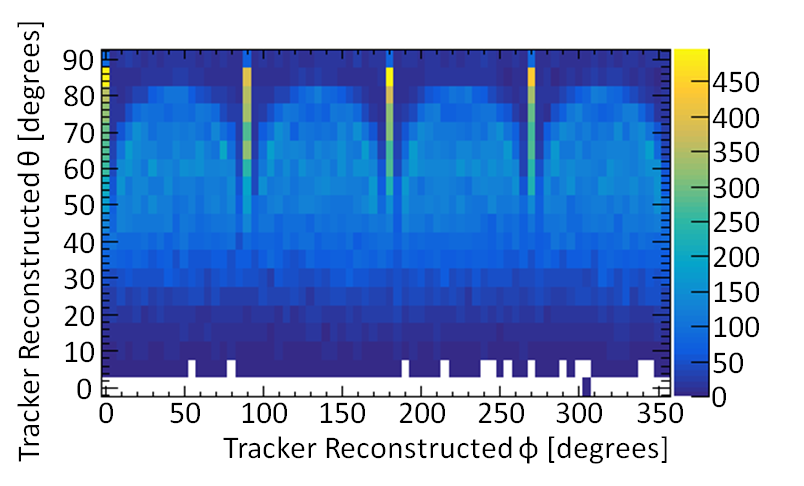
\includegraphics[width=0.9\linewidth]{Chapter6/Figs/Raster/thetaVsPhiSimulatedWithReactor0MedText.png}
  \captionsetup{width=.9\linewidth}
  \caption{}
  \label{subFig:thetaVsPhiSimulatedWithReactor0}
\end{subfigure}%
\begin{subfigure}{.5\textwidth}
  \centering
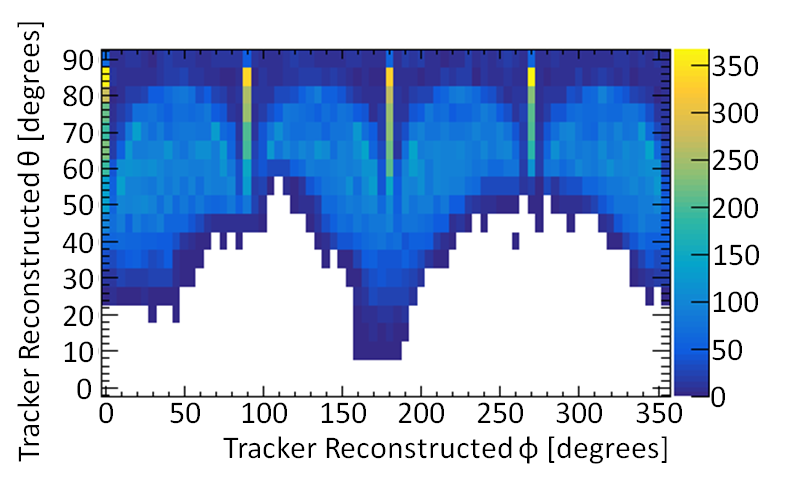
\includegraphics[width=0.9\linewidth]{Chapter6/Figs/Raster/thetaVsPhiSimulatedWithReactor100MedText.png}
  \captionsetup{width=.9\linewidth}
  \caption{}
  \label{subFig:thetaVsPhiSimulatedWithReactor100}
\end{subfigure}
\caption[A side by side comparison of the GEANT4 simulation $\phi$ and $\theta$ distributions.]{A side by side comparison of the GEANT4 simulation $\phi$ and $\theta$ distributions without reactor buildings (seen in (a)) and with reactor buildings (seen in side (b)) using a realistic $\theta$ distribution, based on data taken at Liverpool.}
\label{fig:thetaVsPhiSimulatedWithReactor_0-100}
\end{figure}

\begin{figure}[!h]
 \centering
 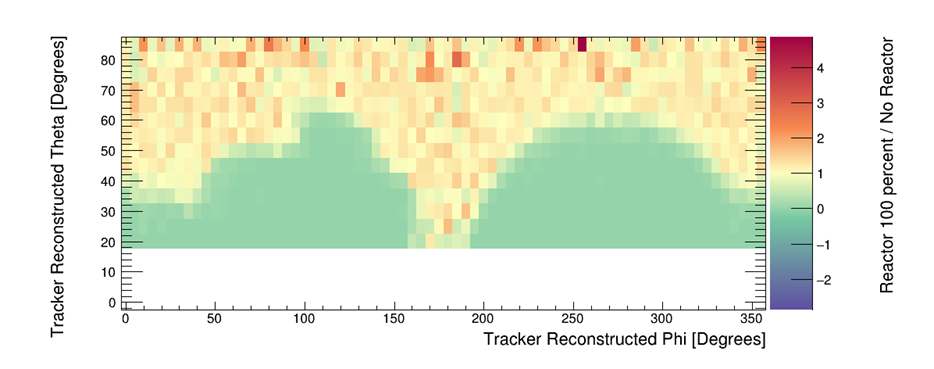
\includegraphics[width=\linewidth]{Chapter5/Figs/wylfaRasterNew/simulatedTrackerReconNoLines.png}
 \captionof{figure}[Ratio of the cosmic muon simulation with and without reactor buildings.]{Ratio of the cosmic muon simulation with and without reactor buildings, highlighting the composite shadow shapes. The area < 17.5$^\circ$ in $\theta$ is ignored for consistency with the Wylfa shadow data set (figure \ref{fig:measuredTrackerReconNoLines}).} 
 \label{fig:simulatedTrackerReconNoLines}
\end{figure}

Once all the outlines are produced they are then overlaid on top of the simulated shadows (figure \ref{fig:simulatedTrackerReconNoLines}) to produce a map of the shadows with corresponding outlines (figure \ref{fig:simulatedTrackerRecon}), which uses the same outline styles as figure \ref{subFig:wylfaTraceStep4}. These outlines are taken and overlaid on top of the measured shadows from the Wylfa reactor site (figure \ref{fig:measuredTrackerReconNoLines}). This gives a map of the Wylfa data set with outlines from each of the expected buildings according to simulation (figure \ref{fig:measuredTrackerRecon}). In this map of the Wylfa data set (figure \ref{fig:measuredTrackerRecon}), the simulated outlines match up well with the measured data, suggesting that the GEANT4 approximate building positions and dimensions (seen in table \ref{tab:simulatedBuildingPositions}) are reasonable. These results are then overlaid using a polar top-down plot as well which is done in figure \ref{fig:wylfaCircular0-37.5Deg_Overlay_Updated}. By doing this it is possible to show that the area of high density viewed in figure \ref{fig:measuredTrackerRecon} most likely corresponds to the reactor core as it lines up with expected location of the near reactor core. 
%\textheight,height=3cm

% \begin{sidewaysfigure}[!h]
%  \centering
%  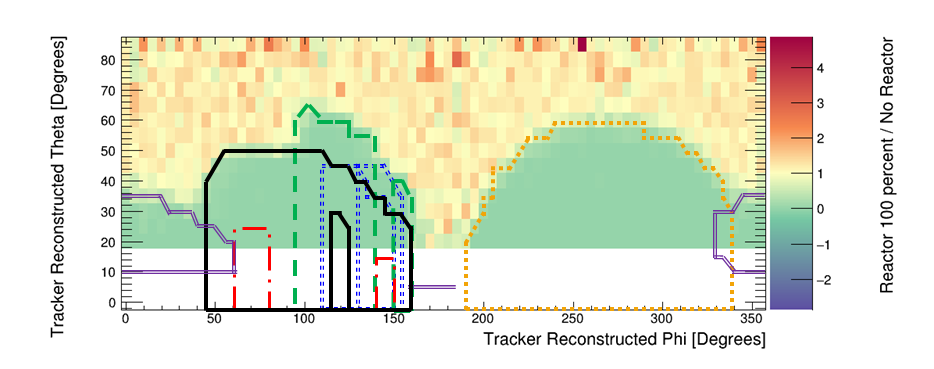
\includegraphics[width=\linewidth]{Chapter5/Figs/wylfaRasterNew/simulatedTrackerRecon.png}
%  \captionof{figure}{Figure \ref{fig:simulatedTrackerReconNoLines} with each simulated reactor building highlighted using lines which correspond to the key in \ref{fig:wylfaTraceStep4}.} 
%  \label{fig:simulatedTrackerRecon}
% \end{sidewaysfigure}

% \begin{sidewaysfigure}[!h]
%  \centering
%  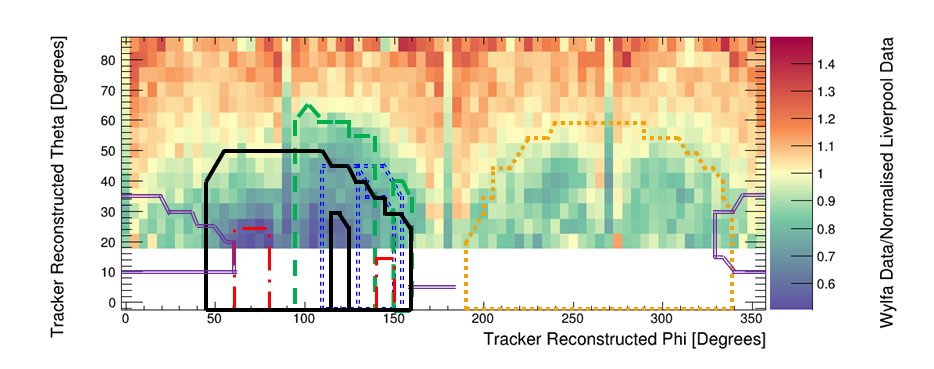
\includegraphics[width=\linewidth]{Chapter5/Figs/wylfaRasterNew/measuredTrackerRecon.png}
%  \captionof{figure}{Figure \ref{fig:measuredTrackerReconNoLines} with each simulated reactor building highlighted using lines which correspond to the key in \ref{fig:wylfaTraceStep4}.} 
%  \label{fig:measuredTrackerRecon}
% \end{sidewaysfigure}



By comparing the map of outlined simulated buildings (figure \ref{fig:simulatedTrackerRecon}) and the map of the outlined measured buildings from Wylfa (figure \ref{fig:measuredTrackerRecon}) the similarities are clear. There are some discrepancies between the simulated and the measured results most noticeably the area of low density between 0$^\circ$ -- 45$^\circ$ in $\phi$ to 30$^\circ$ -- 50$^\circ$ in $\theta$. This is likely caused by other buildings behind the Wylfa Reactor building, which are not simulated because they are not clear and distinct. Also, as they are far away it would be disingenuous to claim that the detector has accurately resolved them. But the overall cosmic muon tomography results (figure \ref{fig:measuredTrackerRecon}) match expectations (figure \ref{fig:simulatedTrackerRecon}) to within 1\,--\,2 5$^\circ$ bins in both $\phi$ and $\theta$. Therefore, it is reasonable to claim that the VIDARR detector can accurately measure and resolve its surroundings at reactor sites with live time data on the order of one hour. This is extremely useful as it prevents the detector from being moved without knowledge of the detector operator. This was achieved despite not having a dedicated cosmic muon mode for the Wylfa data set. Based on the results of this work, the VIDARR detector will have a cosmic muon mode and as such by switching to this cosmic mode for one hour a week it should be possible to determine any significant movement ($\sim 5\,\textrm{m}$ in $x$ or $y$) and thus deter tampering by physical movement of the detector. It is also worth noting that the segmentation being $4\,\textrm{cm} \times 1\,\textrm{cm}$ is fortuitous for cosmic muon tomography. As the range for $\theta$ is (0$^\circ$ -- 90$^\circ$) four times finer than the range for $\phi$ (0$^\circ$ -- 360$^\circ$) therefore having segmentation that is able to resolve these to the same standard is a significant advantage when imaging the surroundings. And it is also worth noting the advantage that Liverpool and Wylfa share the same latitude (53.4$^\circ$) thus making the Liverpool control data especially useful. %in latitude shared by both Liverpool and Wylfa of 53.4$^\circ$ without such a good control data set it is possible the shadows would not have been as clearly resolved. 

\begin{sidewaysfigure}[!h]
  \centering
    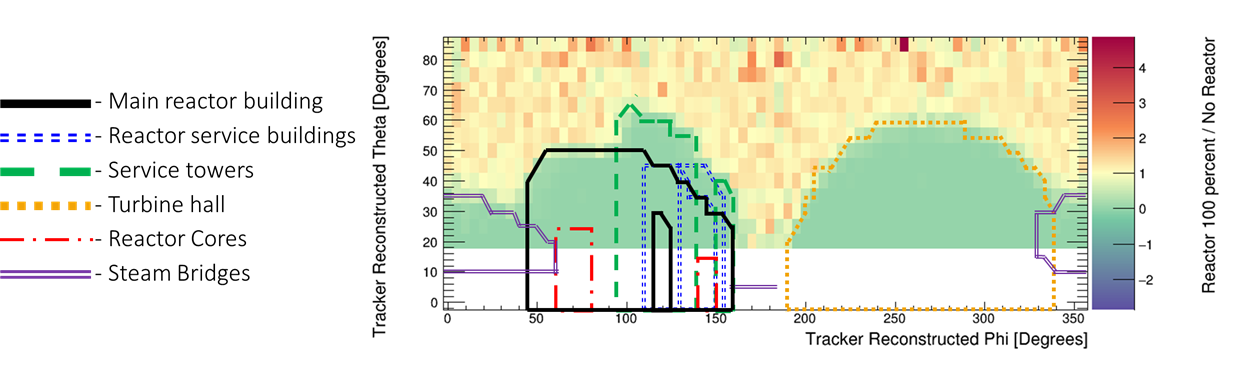
\includegraphics[width=1\linewidth]{Chapter6/Figs/Raster/wylfaSimulatedShadowsWithKey.png}
    \caption[Ratio of simulated buildings (100\,\% concrete).]{Ratio of simulated buildings (100\,\% concrete) and no simulated buildings each component that leads to the composite shadow has been outlined with a key.}
  \label{fig:simulatedTrackerRecon}
    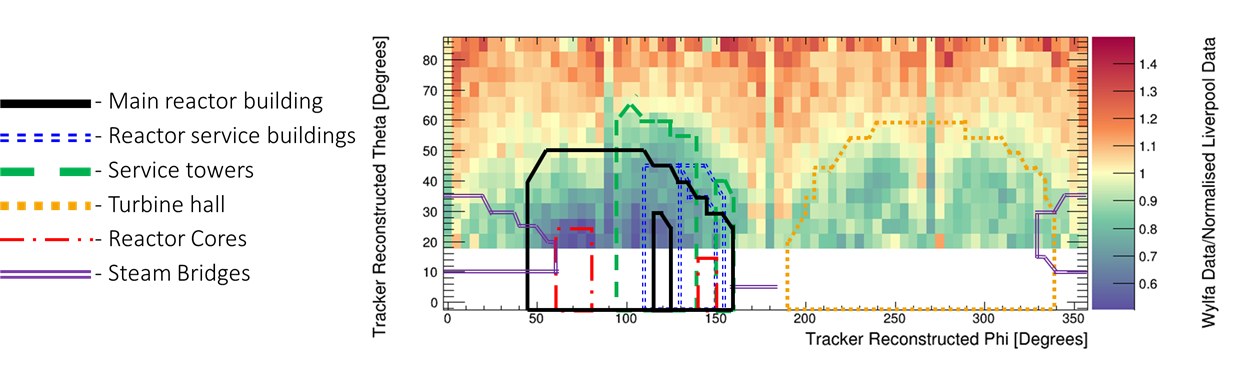
\includegraphics[width=1\linewidth]{Chapter6/Figs/Raster/wylfaMeasuredShadowsWithKey.png}
    \caption[Ratio of Wylfa data and normalised Liverpool data.]{Ratio of Wylfa data and normalised Liverpool data with the outlines from simulation superimposed. The shadows match expectations well.}
  \label{fig:measuredTrackerRecon}
\end{sidewaysfigure}

\clearpage

\begin{figure}[!h]
 \centering
 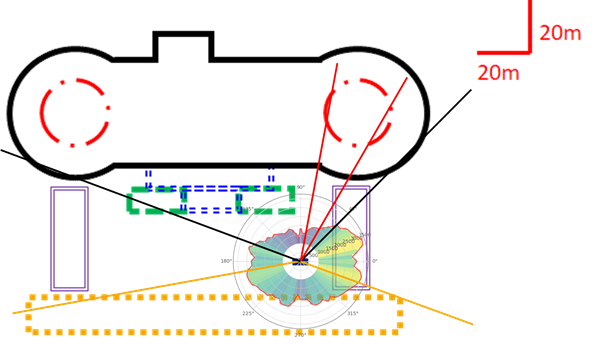
\includegraphics[width=\linewidth]{Chapter5/Figs/wylfaRasterNew/wylfaCircular0-37.5Deg_Overlay_Updated.png}
 \captionof{figure}[Top down Wylfa trace with an updated polar $\phi$ histogram.]{Top down Wylfa trace with an updated polar $\phi$ histogram to show how much more accurate the boundaries are now that the building occlusions in $\phi$ and $\theta$ are better understood.}  
 \label{fig:wylfaCircular0-37.5Deg_Overlay_Updated}
\end{figure}

\section{Cosmic Tracker Uncertainties}\label{sec:cosmicTrackerUncertainties}
The cosmic muon results from figures \ref{fig:simulatedTrackerRecon}, \ref{fig:measuredTrackerRecon} and \ref{fig:wylfaCircular0-37.5Deg_Overlay_Updated} are highly promising. However, there are some potential issues with regards to the bin migration previously mentioned, especially in figures \ref{fig:measuredTrackerReconNoLines} and \ref{fig:measuredTrackerRecon} where the vertical lines at $\phi$ = 0$^\circ$, $\phi$ = 90$^\circ$, $\phi$ = 180$^\circ$, $\phi$ = 270$^\circ$ are still visible. The uncertainties can be quantified to some extent, but the limits are due to the detector's geometry and segmentation rather than the analysis. In order to quantify the uncertainty of the tracker and detector 10$^6$ cosmic muon particles were simulated in GEANT4 with a $\phi$ of  135$^\circ$ and $\theta$ of 45$^\circ$. A random spot is then chosen in the detector and then they are back-projected by 3\,m. The generated distribution of which can be seen in figure \ref{fig:sideABGen_PVsT_135_45}. The reconstruction then fits and produces the tracks (figure \ref{fig:trackedABWithDead}). When comparing the tracker results from figure \ref{fig:trackedABWithDead} with the generated distributions in figure \ref{fig:sideABGen_PVsT_135_45} there is only a minimal difference which is unsurprising, as the efficiency is 98.6\,\% for the reconstruction. 

\begin{figure}[!h]
\centering
\begin{subfigure}{.5\textwidth}
  \centering
  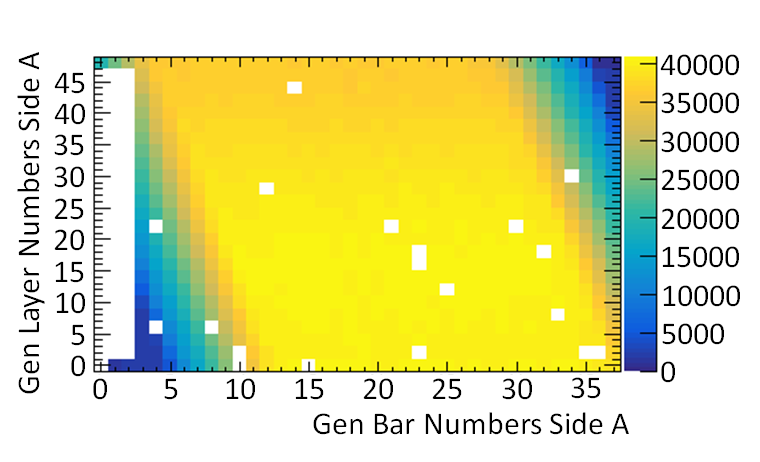
\includegraphics[width=\linewidth]{Chapter6/Figs/Raster/sideAGen_PVsT_135_45MedText.png}
  \captionsetup{width=.9\linewidth}
  \caption{}
  \label{subFig:sideAGen_PVsT_135_45}
\end{subfigure}%
\begin{subfigure}{.5\textwidth}
  \centering
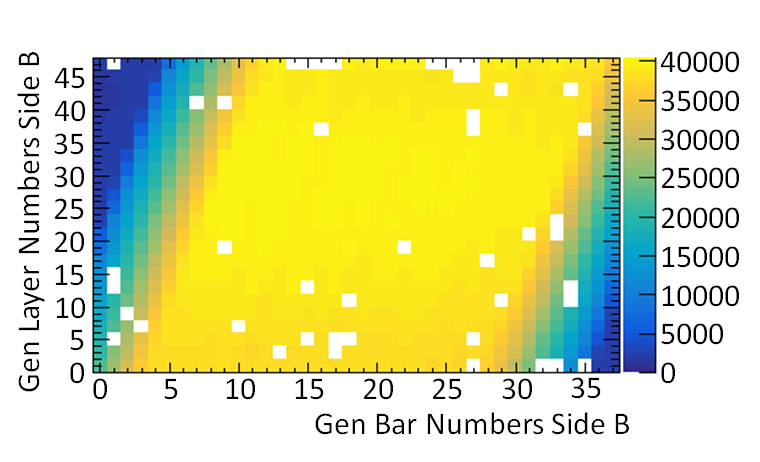
\includegraphics[width=\linewidth]{Chapter6/Figs/Raster/sideBGen_PVsT_135_45MedText.png}
  \captionsetup{width=.9\linewidth}
  \caption{}
  \label{subFig:sideBGen_PVsT_135_45}
\end{subfigure}
\caption[The generated hits in GEANT4 for $\phi$ = 135$^\circ$ and $\theta$ = 45$^\circ$.]{The generated hits in GEANT4 for $\phi$ = 135$^\circ$ and $\theta$ = 45$^\circ$ with dead and uninstrumented channels taken into account. Side A is shown in (a). Side B is shown in (b).}
\label{fig:sideABGen_PVsT_135_45}
\end{figure}

\begin{figure}[!h]
\centering
\begin{subfigure}{.5\textwidth}
  \centering
  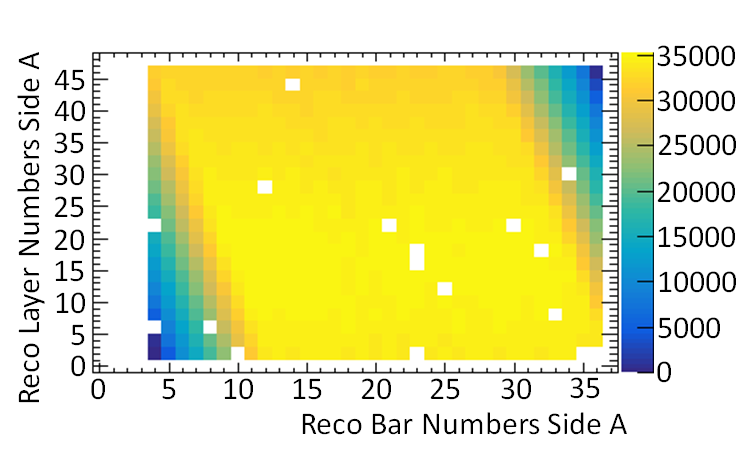
\includegraphics[width=\linewidth]{Chapter6/Figs/Raster/trackedAWithDeadMedText.png}
  \captionsetup{width=.9\linewidth}
  \caption{}
  \label{subFig:trackedAWithDead}
\end{subfigure}%
\begin{subfigure}{.5\textwidth}
  \centering
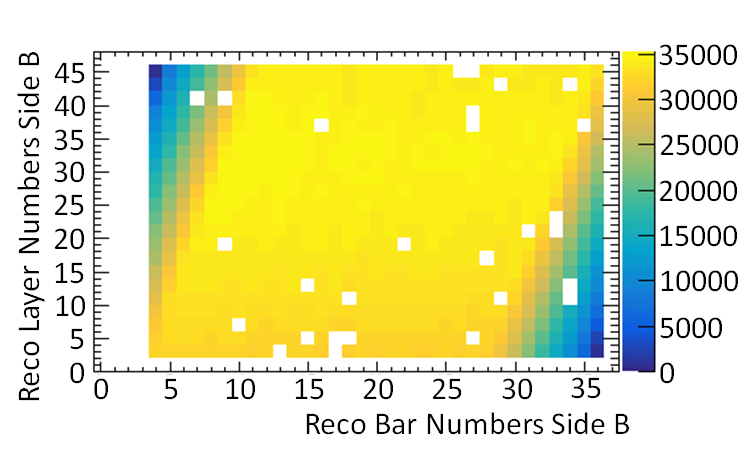
\includegraphics[width=\linewidth]{Chapter6/Figs/Raster/trackedBWithDeadMedText.png}
  \captionsetup{width=.9\linewidth}
  \caption{}
  \label{subFig:trackedBWithDead}
\end{subfigure}
\caption[Tracker reconstructed hits for the $\phi$ = 135$^\circ$ and $\theta$ = 45$^\circ$.]{Tracker reconstructed hits for the $\phi$ = 135$^\circ$ and $\theta$ = 45$^\circ$, the tracker is not thrown off by the dead channels or the fiducial channels. It reconstructs the simulated distribution well. Side A is shown in (a). Side B is shown in (b).}
\label{fig:trackedABWithDead}
\end{figure}

The reconstructed $\phi$ and $\theta$ distributions are shown in figure \ref{fig:pVsTWithDeadLog} where about $\sim$ 50\,\% of the data is reconstructed in the $\phi = 135^\circ$, $\theta = 45^\circ$ bin. However, in figure \ref{fig:pVsTWithDeadLog} there is significant smearing at both angles. The smearing in $\phi$ is roughly even with smearing equally likely to be both above and below the generated value of $\phi = 135^\circ$. More interesting is the smearing in $\theta$ which is more likely to smear above than below the generated value of $\theta = 45^\circ$. This is a result of how cosmic muon events propagate in the detector and the nature of the fiducialisation in the detector. In figure \ref{fig:badFitNoFiducial}, an example event shows how the reconstruction ignores the noise and fits signal. But when the detector is fiducialised as in figure \ref{fig:badFitWithFiducial} the narrower detector results in noise hits being considered part of the cosmic muon event. This migrates the event to a higher value of $\theta$ and a lower value of $\phi$. Even if the noise is properly excluded there is insufficient information to accurately determine the values of $\phi$ and $\theta$ as the event in \ref{fig:badFitWithFiducial} only extends over two bars. Also, due to timing and electronic effects, sometimes real-world cosmic muon events will have large gaps in the track so excluding events like \ref{fig:badFitWithFiducial} is not feasible. As cosmic muon events propagate downwards through the detector, the fitter is more likely to fit above expected $\theta$ values rather than below as corner clipping events are likely to be narrower than the originating muon event. This is also a key component of the bin migration previously mentioned. 

\begin{figure}[!h]
 \centering
 \includegraphics[width=0.7\linewidth]{Chapter5/Figs/cosmicTrackerUncertainties/pVsTWithDeadLog.png}
 \captionof{figure}[Tracker reconstructed $\phi$ and $\theta$ for simulated $\phi$ = 135$^\circ$ and $\theta$ = 45$^\circ$.]{Tracker reconstructed $\phi$ and $\theta$ for simulated $\phi$ = 135$^\circ$ and $\theta$ = 45$^\circ$. The most likely value to be reconstructed is $\phi$ = 135$^\circ$ and $\theta$ = 45$^\circ$ (representing $\sim$ 55\,\% of the reconstruction) but there is significant smearing in both angles. Efficiency is 98.6\,\%.} 
 \label{fig:pVsTWithDeadLog}
\end{figure}

\begin{figure}[!h]
 \centering
 \includegraphics[width=\linewidth]{Chapter6/Figs/Raster/135,45_85,60__noDead_updatedAxis_cosmicCandidate195939MedText.png}
 \captionof{figure}[Example candidate cosmic event, GEANT4 data $\phi$ = 135$^\circ$ and $\theta$ = 45$^\circ$]{Example candidate cosmic event from the generated GEANT4 data for $\phi$ = 135$^\circ$ and $\theta$ = 45$^\circ$ with all channels. The reconstruction correctly ignores the noise and fits the signal.} 
 \label{fig:badFitNoFiducial}
\end{figure}

\begin{figure}[!h]
 \centering
 \includegraphics[width=\linewidth]{Chapter6/Figs/Raster/135,45_85,60__withDead_updatedAxis_cosmicCandidate195939MedText.png}
 \captionof{figure}[Example candidate cosmic event, GEANT4 data $\phi$ = 135$^\circ$ and $\theta$ = 45$^\circ$, with bad channels.]{Example candidate cosmic event from figure \ref{fig:badFitNoFiducial} with fiducial exclusion, dead channels, and uninstrumented channels taken into account. The tracker tries to fit the signal but due to corner clipping nature of the event the fitting on side A has failed and fits to $\phi$ = 85$^\circ$ and $\theta$ = 60$^\circ$ instead of $\phi$ = 135$^\circ$ and $\theta$ = 45$^\circ$. } 
 \label{fig:badFitWithFiducial}
\end{figure}

Fitting the smeared $\phi$ and $\theta$ distribution yields inaccurate fits which is unsurprising considering how significant the smearing is in figure \ref{fig:pVsTWithDeadLog}. For both the $\chi^2$/DOF is > 170 which is far above acceptable levels (see figures \ref{fig:fittingPhiWithDead}, \ref{fig:fittingThetaWithDead}). In both cases, the function attempted to be fitted is a double Gaussian function with a ``noise'' Gaussian function to take into account the smearing and a Gaussian attempting to fit the signal. For the fitted $\phi$ distribution the mean angle of the signal was 136.288$^\circ$ with a signal $\sigma$ of 0.728$^\circ$. Considering the spread of the $\phi$ distribution is significant, these values are reasonable but it is clear from figure \ref{fig:fittingPhiWithDead} that the peak of the signal distribution is not fitted well. For the fitted $\theta$ distribution the mean angle of the signal was 45.1275$^\circ$ with a signal $\sigma$ of 0.3524$^\circ$. These values are very good for the $\theta$ distribution and whilst the fit in figure \ref{fig:fittingThetaWithDead} has large $\chi^2$/DOF, the peak of the signal distribution is much closer than in $\phi$ and the noise ``shoulder'' in $\theta$ seems more accurately characterised. It is not surprising that the fitting for $\theta$ is more accurate as the segments for the detector are four times wider than they are tall. 


\begin{figure}[!h]
\centering
\begin{minipage}{.45\textwidth}
  \centering
  \includegraphics[width=\linewidth]{Chapter6/Figs/Raster/phiFittedNewProportionsMedText.png}
  \captionof{figure}[Double Gaussian fitted to the reconstructed tracker $\phi$ values.]{Double Gaussian fitted to the reconstructed tracker $\phi$ values when simulating $\phi$ = 135$^\circ$ and $\theta$ = 45$^\circ$ exclusively. The $\chi^2$/DOF is 181.31 showing a poor fit which is largely due to segmentation effects. signal mean = 136.288, signal $\sigma$ 0.728, noise mean = 140.101, noise $\sigma$ 7.819.} 
  \label{fig:fittingPhiWithDead}
\end{minipage}%
\qquad
\begin{minipage}{.45\textwidth}
  \centering
  \includegraphics[width=\linewidth]{Chapter6/Figs/Raster/thetaFittedNewProportionsMedText.png}
  \captionof{figure}[Double Gaussian fitted to the reconstructed tracker $\theta$ values.]{Double Gaussian fitted to the reconstructed tracker $\theta$ values when simulating $\phi$ = 135$^\circ$ and $\theta$ = 45$^\circ$ exclusively. The $\chi^2$/DOF is 172.758 showing a poor fit which is largely due to segmentation effects. Signal mean = 45.1275, signal $\sigma$ = 0.3524, noise mean = 46.8153, noise $\sigma$ = 1.6294.}
  \label{fig:fittingThetaWithDead}
\end{minipage}
\end{figure}


% \begin{figure}[!h]
%  \centering
%  \includegraphics[width=\linewidth]{Chapter5/Figs/cosmicTrackerUncertainties/fittingPhiWithDead.png}
%  \captionof{figure}{} 
%  \label{fig:fittingPhiWithDead}
% \end{figure}

% \begin{figure}[!h]
%  \centering
%  \includegraphics[width=\linewidth]{Chapter5/Figs/cosmicTrackerUncertainties/fittingThetaWithDead.png}
%  \captionof{figure}{} 
%  \label{fig:fittingThetaWithDead}
% \end{figure}

It is possible to mitigate the effect of these corner clipping events by requiring a large number of bar segments to be hit per side. In figure \ref{fig:pVsT135FidFix_20barCutPerSide} a requirement of 20 bars being hit for each side is introduced. When comparing figure \ref{fig:pVsTWithDeadLog} which requires four bars to be hit per side and figure \ref{fig:pVsT135FidFix_20barCutPerSide} which requires 20 bars to be hit per side, the spread has been greatly reduced. However, this selection criterion reduces the efficiency from 98.6\,\% to 68.9\,\%. Additionally this effect does not affect all events equally, events with a lower value of $\theta$ will be more likely to be removed. As a result, when using this selection criterion on the measured data in figure \ref{fig:20CutRatioWylfaDivLiv}, the shadows become less clear as $\theta$ decreases. This highlights the paradox between increasing precision and increasing accuracy for this particular data set. Cosmic muon events that cross the corner of the detector are the most useful for cosmic muon tomography at low angles of $\theta$ so a shadow analysis that uses these events will be more accurate. But these are also the events that will have the most smearing and so will reduce precision. In conclusion, the effects introduced by using smaller events are a significant cause for bin migration but trying to mitigate this effect degrades the shadows more than it solves the bin migration issue. Therefore, it is better to keep as many events as possible and take the ratio using a control data set rather than try to find a golden selection. As figure \ref{fig:20CutRatioWylfaDivLiv} shows the attempt to find more precise data does not improve the shadows.

\begin{figure}[!h]
 \centering
 \includegraphics[width=0.7\linewidth]{Chapter5/Figs/cosmicTrackerUncertainties/pVsT135FidFix_20barCutPerSide.png}
 \captionof{figure}[Tracker reconstructed $\phi$ and $\theta$ but with a $<$ 20 hits threshold for each side.]{Tracker reconstructed $\phi$ and $\theta$ but with all events that have $<$ 20 hits for side A, and $<$ 20 hits for side B removed. This greatly improves the distribution and reduces smearing. However, efficiency is only 68.9\,\% $\sim$ 30\,\% lower than with a 4 bar cut on either side.} 
 \label{fig:pVsT135FidFix_20barCutPerSide}
\end{figure}

\begin{figure}[!h]
 \centering
 \includegraphics[width=\linewidth]{Chapter6/Figs/simulatedMeasuredCut20Bars.png}
 \captionof{figure}[Ratio of Liverpool and Wylfa cosmic muon data sets with 20 bar threshold cuts.]{How the ratio of the Liverpool and Wylfa data sets looks when a 20 bar cut per side is used. Instead of a 4 bar cut (See figures \ref{fig:measuredTrackerReconNoLines} and \ref{fig:measuredTrackerRecon}). The shadows for both the turbine hall (centred around $\phi$ = 270$^\circ$) and reactor buildings (centred around $\phi$ = 90 $^\circ$) are less accurately resolved now. Despite the more precise angle reconstruction, the number of side on events has been greatly reduced and as those are the most useful events for this tomography the outlines have greatly degraded.}
 \label{fig:20CutRatioWylfaDivLiv}
\end{figure}

%\clearpage
%\vspace{5cm}
\section{Using Simulated Data as Control Data}\label{sec:usingSimulatedDataAsControlData}
Another possible alternative to using the Liverpool data set as control is to use simulated data as a control data set. However, this has major limitations even when using a $\theta$ distribution which is derived from measured data. The overall $\theta$ distribution for simulated data can be seen in figure \ref{fig:thetaGenRecoCryAndNorm} which is a good approximation to the measured data in figure \ref{fig:measuredThetaWylfaLiverpool}. The overall $\phi$ and $\theta$ distribution for the simulated data can be seen in figure \ref{fig:mc_PvsT} which looks similar to the Liverpool and Wylfa data sets. Providing the $\theta$ distribution is accurate and the GEANT4 simulation correctly models the atmospheric smearing this distribution should only have detector and segmentation effects smearing the distribution. 

% \begin{figure}[!h]
%  \centering
%  \includegraphics[width=0.7\linewidth]{Chapter5/Figs/UsingSimulatedDataAsControl/mc_theatOnly.png}
%  \captionof{figure}{$\theta$ distribution from simulation using measured data and redistributing to account for potential reconstruction issues and using an exponential tail fit. \hl{This plot needs to be reversed and use the CRY distribution}}
%  \label{fig:mc_thetaOnly}
% \end{figure}

\begin{figure}[!h]
\centering
\begin{subfigure}{.5\textwidth}
  \centering
  \includegraphics[width=\linewidth]{Chapter6/Figs/Raster/thetaGenRecoCryMedText.png}
  \captionsetup{width=.9\linewidth}
  \caption{}
  \label{subFig:thetaGenRecoCry}
\end{subfigure}%
\begin{subfigure}{.5\textwidth}
  \centering
\includegraphics[width=\linewidth]{Chapter6/Figs/Raster/thetaGenRecoCryNormMedText.png}
  \captionsetup{width=.9\linewidth}
  \caption{}
  \label{subFig:thetaGenRecoCryNorm}
\end{subfigure}
\caption[Generated CRY $\theta$ distribution for an altitude of 0\,m (sea-level).]{The generated CRY $\theta$ distribution for an altitude of 0\,m (sea-level) and latitude of 53.4$^\circ$ (The latitude of Wylfa and Liverpool). In (a) the generated and reconstructed are compared and in (b) the generated and reconstructed are normalised. The overall shape is very well preserved by the detector and tracker.}
\label{fig:thetaGenRecoCryAndNorm}
\end{figure}

\begin{figure}[!h]
\centering
\begin{subfigure}{.5\textwidth}
  \centering
  \includegraphics[width=\linewidth]{Chapter6/Figs/Raster/thetaWylfaLiverpoolNewMedText.png}
  \captionsetup{width=.9\linewidth}
  \caption{}
  \label{subFig:measuredThetaWylfaLiv}
\end{subfigure}%
\begin{subfigure}{.5\textwidth}
  \centering
\includegraphics[width=\linewidth]{Chapter6/Figs/Raster/thetaWylfaLiverpoolNewNormMedText.png}
  \captionsetup{width=.9\linewidth}
  \caption{}
  \label{subFig:measuredThetaWylfaLivNorm}
\end{subfigure}
\caption[Measured $\theta$ distributions at Wylfa and Liverpool.]{The measured $\theta$ distributions at Wylfa and Liverpool, the Liverpool data set is larger (visible in (a)) but when normalised it is clear how similar the two distributions are in (b).}
\label{fig:measuredThetaWylfaLiverpool}
\end{figure}

\begin{figure}[!h]
 \centering
 \includegraphics[width=0.7\linewidth]{Chapter6/Figs/phiVsThetaCryReco.png}
 \captionof{figure}[Tracker reconstructed ($\phi$,$\theta$) distribution using CRY distribution.]{Tracker reconstructed ($\phi$,$\theta$) distribution using a flat $\phi$ distribution (0$^\circ$ -- 360$^\circ$) and the CRY $\theta$ distribution \cite{ieee_cry_2007}.}
 \label{fig:mc_PvsT}
\end{figure}

However, the simulation cannot account for all of the different effects and this is shown by figure \ref{fig:WylfaToMCRatio} where the ratio between the simulated and the measured Wylfa data is taken. In figure \ref{fig:WylfaToMCRatio}, the bin migration is still masking the shadows significantly. Though an indistinct pattern is visible where the reactor buildings are located (between $\phi$ values of 0$^\circ$ -- 180$^\circ$) the turbine hall (between $\phi$ values of 180$^\circ$ -- 360$^\circ$) is no longer discernible. The same effect can be seen when taking the ratio between the simulated and measured Liverpool data in figures \ref{fig:LiverpoolToMCRatio}. The amount of cosmic muon sky occlusion is very minimal in the Liverpool data set but there is still a large discrepancy between that data set and the generated cosmic muon data set. As a result, the Liverpool data set is the preferred control data set to the generated GEANT4 data. 
\\\\ In figure \ref{fig:WylfaToMCRatio} some of the Wylfa shadows are visible. The service tower between $\phi$ values of 90$^\circ$ -- 150$^\circ$ is slightly visible but it is faint. The reactor core / reactor core shielding is still visible however between $\phi$ values of 50$^\circ$ -- 90$^\circ$. This is useful as the reactor core shadow is the only shadow completely hidden by other buildings as the reactor core is housed in the main reactor building. This is highly encouraging as it shows the method using the Liverpool data as a control data set is most likely accurate as the shadow for the reactor core can be independently verified as neither the reactor core nor service tower are visible in figure \ref{fig:LiverpoolToMCRatio}. The distribution difference between the Liverpool control data and the generated GEANT4 control data seen in figure \ref{fig:LiverpoolToMCRatio} is difficult to fix. The difference in scattering and showering would require potentially a full atmospheric simulation. Considering the amount of atmosphere that would need to be simulated this is largely infeasible. Whilst CRY has made good approximations from measured data and is very close to measured data (as shown by comparing \ref{subFig:thetaGenRecoCryNorm} and \ref{subFig:measuredThetaWylfaLivNorm}) more detailed simulations and potentially different approaches to simulating large areas may be required to produce simulated distributions which serve as effective control data sets. While this cannot be achieved within a reasonable time scale for this project, it is nevertheless an interesting avenue for future work and the technique demonstrated by figure \ref{fig:WylfaToMCRatio} shows promise. 

\begin{figure}[!h]
 \centering
 \includegraphics[width=\linewidth]{Chapter6/Figs/WylfaCryRatioPartialOutlines.png}
 \captionof{figure}[Ratio of $\phi$ and $\theta$ of the Wylfa data set against the generated normalised GEANT4 data set.]{The ratio of $\phi$ and $\theta$ of the Wylfa data set against the generated normalised GEANT4 data set (see figure \ref{fig:mc_PvsT}). The turbine hall is no longer visible, the service tower is still partially visible between $\phi$ values 90$^\circ$ -- 150$^\circ$. But the reactor core area between $\phi$ values of 50$^\circ$ -- 90$^\circ$ is still clearly visible. }
 \label{fig:WylfaToMCRatio}
\end{figure}

\begin{figure}[!h]
 \centering
 \includegraphics[width=\linewidth]{Chapter6/Figs/LiverpoolCryRatioPartialOutlines.png}
 \captionof{figure}[Ratio of $\phi$ and $\theta$ of the Liverpool data set against the generated normalised GEANT4 data set.]{The ratio of $\phi$ and $\theta$ of the Liverpool data set against the generated normalised GEANT4 data set (see figure \ref{fig:mc_PvsT}). There are no clear shadows. There is a large difference between the generated data set and measured data set. This is likely due to the difference in scattering between GEANT4 and the real-world scattering.}
 \label{fig:LiverpoolToMCRatio}
\end{figure}


% \begin{figure}[!h]
% \centering
% \begin{minipage}{.45\textwidth}
%   \centering
%   \includegraphics[width=\linewidth]{Chapter5/Figs/UsingSimulatedDataAsControl/WylfaToMCRatio.png}
%   \captionof{figure}{Ratio of Wylfa to GEANT4 simulated data the bin migration hides the shadows \hl{Needs to be redone with Cry Distribution + reformatting}} 
%   \label{fig:WylfaToMCRatio}
% \end{minipage}%
% \qquad
% \begin{minipage}{.45\textwidth}
%   \centering
%   \includegraphics[width=\linewidth]{Chapter5/Figs/UsingSimulatedDataAsControl/WylfaToMCRatio0-2.png}
%   \captionof{figure}{Ratio of Wylfa to GEANT4 simulated data restricted to a maximum of 2 the bin migration still causes the tops of the shadows to be difficult to determine. \hl{Needs to be redone with Cry Distribution + reformatting}}
%   \label{fig:WylfaToMCRatio0-2}
% \end{minipage}
% \end{figure}

% \begin{figure}[!h]
% \centering
% \begin{minipage}{.45\textwidth}
%   \centering
%   \includegraphics[width=\linewidth]{Chapter5/Figs/UsingSimulatedDataAsControl/LiverpoolToMCRatio.png}
%   \captionof{figure}{Ratio of Liverpool to GEANT4 simulated data the bin migration dominates \hl{Needs to be redone with Cry Distribution + reformatting}.} 
%   \label{fig:LiverpoolToMCRatio}
% \end{minipage}%
% \qquad
% \begin{minipage}{.45\textwidth}
%   \centering
%   \includegraphics[width=\linewidth]{Chapter5/Figs/UsingSimulatedDataAsControl/LiverpoolToMCRatio0-2.png}
%   \captionof{figure}{Ratio of the Liverpool to GEANT4 simulated data restricted to a maximum of 2. Unexpected areas below blocked incidence of 1 are visible even though there is nothing at the Liverpool site that could cause such shadows to occur. \hl{Needs to be redone with Cry Distribution + reformatting}.}
%   \label{fig:LiverpoolToMCRatio0-2}
% \end{minipage}
% \end{figure}

% Cosmic muon tomography is split into two distinct types two sided and one sided. Two sided cosmic muon is preferred if it is feasible this is because both attenuation and scattering can be measured when using this technique. The effect of the cosmic muon scattering can be seen in figure \ref{fig:twoSidedCosmicMuonTomographySchults} the cosmic muon which travel through the dense object will scatter more than the cosmic muon that don't. By making coincident measurements of the cosmic muon it is possible to find vertices using this method. This method is extremely powerful but can only be used for smaller objects in most cases. 
% \\\\ For larger objects one sided cosmic muon tomography has to be used. An example of what one sided cosmic muon tomography looks like can be seen in figure \ref{fig:oneSidedCosmicMuonExample} when there is an object that can attenuate cosmic muon then the number of cosmic muon will decrease in the direction of the object being imaged. This method cannot measure scattering or vertices however that is still sufficient in many cases such as the imaging done by the DIAPHANE collaboration seen in figure  \ref{fig:diaphaneStructualImaging}. Which uses 4 different locations to image the La Soufriere of Guadeloupe dome and measure the density for volcanic observations \cite{Marteau_2017}.
% \\\\Need to cite \cite{ANASTASIO2013423} talking about Mu-Ray and SiPms blah

% In order to find the approximate position of detector at the Wylfa site Google Maps was used as the detector's container was large enough to be seen by the Google Maps satellite. The initial step can be seen in figure \ref{fig:wylfaTraceStep0}. Once the detector position has been identified a rough trace of the buildings is then performed with basic shapes seen in figure \ref{fig:wylfaTraceStep1}. However because the site buildings are taller than the detector by quite a significant margin the base position of the buildings does not match the top position of the buildings seen in the google maps. In figure \ref{fig:wylfaTraceStep2} key areas of the site buildings are used as reference points to so that the base of the buildings is more accurately represented. Finally the background and any connecting lines are removed in figure \ref{fig:wylfaTraceStep4} which shows the final Wylfa trace.  

% \begin{figure}[!h]
%  \centering
%  \includegraphics[width=\linewidth]{Chapter5/Figs/Raster/wylfaTraceStep0.png}
%  \captionof{figure}{The detector at the Wylfa reactor site.} 
%  \label{fig:wylfaTraceStep0}
% \end{figure}

% \begin{figure}[!h]
%  \centering
%  \includegraphics[width=\linewidth]{Chapter5/Figs/Raster/wylfaTraceStep1.png}
%  \captionof{figure}{Basic shapes are overlaid on top of the detector and site buildings.} 
%  \label{fig:wylfaTraceStep1}
% \end{figure}

% \begin{figure}[!h]
%  \centering
%  \includegraphics[width=\linewidth]{Chapter5/Figs/Raster/wylfaTraceStep2.png}
%  \captionof{figure}{reference points are used to offset the tall site buildings closer to the base of the buildings. This is done to take into account the angle of the google maps satellite.} 
%  \label{fig:wylfaTraceStep2}
% \end{figure}

% \begin{figure}[!h]
%  \centering
%  \includegraphics[width=\linewidth]{Chapter5/Figs/Raster/wylfaTraceStep4.png}
%  \captionof{figure}{Finally the background of the reactor site is removed and we are left with a trace of the reactor site.} 
%  \label{fig:wylfaTraceStep4}
% \end{figure}

% The cosmic muon tracker has several steps. First if fewer than 8 bars are hit above 0.7\,MeV the event is discarded. Then if either side has less than 4 hits > 0.7\,MeV the event is discarded. Then the top and bottom hit is found for each side of the detector from this a basic approximation of the gradient is found. This provides a starting point for the fitter on each side, this leads to the initial fit where all of the events above the 0.7\,MeV threshold are fitted, this is preferred over clustering as it includes low angled $\theta$ cosmic muon that clustering often removes. Then any hits that are 2 bars away from the track are discarded, and any lone hits that are 8 bars away from any other hits are also removed then the second fit is applied. Then any hits within one bar of the fitted track are then re-accepted as part of the track. Any lone hits to within a radius of 4 bars from the track are once again removed. This then leads to the third and final fit, which is very fast as the approximation by the second fit is usually quite close to third fit. Then any track which has less than 4 hits per side is then rejected. Finally if 50\,\% of the track energy is missing in either side the event is also removed, this is because under such circumstances it is likely that a second cosmic event is inside the detector or a shower has produced multiple tracks. In figure \ref{fig:3000ExampleEvent} it can be seen that even with a large number of noise hits ($\sim$ 10 noise hits per side) the fitter has still accurately reconstructed the event. 
 
% \begin{figure}[!h]
%  \centering
%  \includegraphics[width=\linewidth]{Chapter5/Figs/Raster/testEventNewScheme.png}
%  \captionof{figure}{An example event from the Wylfa deployment the cosmic enters through the top of the detector and exits through the bottom. The signal that the tracker has identified is shown in orange. The hits the tracker discards are shown in yellow. The un-instrumented block on side A is shown in grey. The dead channels are shown in dark purple. The channels removed for fiducial purposes are shown in light blue.} 
%  \label{fig:3000ExampleEvent}
% \end{figure}

% Using this fitter the data from both the 2014 -- 2015 Wylfa deployment, figure \ref{fig:pVsTWylfaReversed}, and the 2015 -- 2018 deployment at Liverpool, figure \ref{fig:pVsTLiverpoolReversed}, can be analysed for tomographic purposes. Both of these data sets have shadows in them, the shadows in the Liverpool data set are significantly fainter than the shadows in the Wylfa data as the buildings at Wylfa are mostly comprised of concrete where as the buildings at Liverpool are mostly comprised of brick, glass, and steel. In the Liverpool data set the shadows are only visible at very shallow angles of $\theta$ due to the difference in building densities. At Liverpool whilst other buildings are visible in the data set the old accelerator hall is the most visible component which is highlighted in figure \ref{fig:liverpoolCirShadows}. However these shadows are only visible from 0$^{\circ}$ $\theta$ -- 17.5$^{\circ}$ $\theta$, at angles higher than 17.5 $^{\circ}$ $\theta$ the shadows are too faint. 
% \begin{figure}[!h]
%  \centering
%  \includegraphics[width=0.8\linewidth]{Chapter5/Figs/Raster/pVsTWylfaReversed.png}
%  \captionof{figure}{Measured $\theta$ and $\phi$ from the cosmic muon from the Wylfa deployment, the reactor is at $\sim$ 90$^{\circ}$. The turbine hall is at $\sim$ 270$^{\circ}$.} 
%  \label{fig:pVsTWylfaReversed}
% \end{figure}

% \begin{figure}[!h]
%  \centering
%  \includegraphics[width=0.8\linewidth]{Chapter5/Figs/Raster/pVsTLiverpoolReversed.png}
%  \captionof{figure}{Measured $\theta$ and $\phi$ from the cosmic muon from the Liverpool deployment.} 
%  \label{fig:pVsTLiverpoolReversed}
% \end{figure}

% \begin{figure}[!h]
%  \centering
%  \includegraphics[width=0.8\linewidth]{Chapter5/Figs/Raster/liverpoolShadows.png}
%  \captionof{figure}{Measured $\theta$ and $\phi$ from the cosmic muon from the Liverpool deployment shown with the map of Liverpool in the background. The major dip at highlighted by the black lines is due to the accelerator hall at Liverpool.} 
%  \label{fig:liverpoolCirShadows}
% \end{figure}

% The shadows in the Wylfa data are much clearer, seen in figures \ref{fig:WylfaSlice0-57.5} and \ref{fig:wylfaTraceAbove32.5} shows $\phi$ from 0$^{\circ}$ $\theta$ -- 57.5$^{\circ}$ $\theta$ the shadows are clearly visible from both the turbine hall highlighted in-between the orange lines and the reactor buildings shown in-between the black lines. The shape however does not accurately represent the size of the reactor footprint or the width of the turbine hall. This is due to the angles of cosmic muon that are being attenuated by the buildings. In order to accurately quantify the width of the reactor building cosmic muon from lower angles must be considered in figures \ref{fig:WylfaSlice0-37.5} and \ref{fig:wylfaTraceAbove52.5}  show $\phi$ from 0$^{\circ}$ $\theta$ -- 37.5$^{\circ}$ $\theta$ this now gives a much more accurate estimate for the size of the reactor building and $phi$. The size of the turbine hall in $\phi$ is less accurate due to the corrugated steel the turbine hall is constructed with, this means the far edge of the turbine hall is hard to discern which can be seen in figure \ref{fig:wylfaTraceAbove52.5}.

% \begin{figure}[!h]
% \centering
% \begin{subfigure}{.5\textwidth}
%   \centering
%   \includegraphics[width=\linewidth]{Chapter5/Figs/Raster/linReversedWylfaSlice0-57.5.png}
%   \captionsetup{width=.9\linewidth}
%   \caption{Linear histogram showing the dips in the shadows from the shadows of the reactor buildings and turbine halls.}
%   \label{subFig:linReversedWylfaSlice0-57.5}
% \end{subfigure}%
% \begin{subfigure}{.5\textwidth}
%   \centering
%   \includegraphics[width=0.765\linewidth]{Chapter5/Figs/Raster/cirReversedWylfaSlice0-57.5.png}
%   \captionsetup{width=.9\linewidth}
%   \caption{Circular histogram showing the dips in the shadows from the shadows of the reactor buildings and turbine halls.}
%   \label{subFig:linReversedWylfaSlice0-57.5}
% \end{subfigure}
% \caption{Histograms showing how the shadows of the reactor buildings and the turbine hall are cast on to the detector from $\theta$ of 0$^\circ$ to 57.5$^\circ$. The Reactor buildings are shown in-between the black lines the turbine hall is shown in-between the orange lines.}
% \label{fig:WylfaSlice0-57.5}
% \end{figure}

% \begin{figure}[!h]
%  \centering
%  \includegraphics[width=\linewidth]{Chapter5/Figs/Raster/cirOverlayReversedWylfaSlice0-57.5.png}
%  \captionof{figure}{The circular distribution of the $\phi$ from a $\theta$ of 0$^\circ$ - 57.5$^\circ$ traced over from google maps and then compared with the documentation given by Wylfa reactor operators. The tower closest to the detector is dominating the distribution of the shadow.} 
%  \label{fig:wylfaTraceAbove32.5}
% \end{figure}

% \begin{figure}[!h]
% \centering
% \begin{subfigure}{.5\textwidth}
%   \centering
%   \includegraphics[width=\linewidth]{Chapter5/Figs/Raster/linReversedWylfaSlice0-37.5.png}
%   \captionsetup{width=.9\linewidth}
%   \caption{Linear histogram showing the dips in the shadows from the shadows of the reactor buildings and turbine halls.}
%   \label{subFig:linReversedWylfaSlice0-37.5}
% \end{subfigure}%
% \begin{subfigure}{.5\textwidth}
%   \centering
%   \includegraphics[width=0.765\linewidth]{Chapter5/Figs/Raster/cirReversedWylfaSlice0-37.5.png}
%   \captionsetup{width=.9\linewidth}
%   \caption{Circular histogram showing the dips in the shadows from the shadows of the reactor buildings and turbine halls.}
%   \label{subFig:cirReversedWylfaSlice0-37.5}
% \end{subfigure}
%  \caption{Histograms showing how the shadows of the reactor buildings and the turbine hall are cast on to the detector from $\theta$ of 0$^\circ$ to 37.5$^\circ$. The Reactor buildings are shown in-between the black lines the turbine hall is shown in-between the orange lines.}
% \label{fig:WylfaSlice0-37.5}
% \end{figure}

% \begin{figure}[!h]
%  \centering
%  \includegraphics[width=\linewidth]{Chapter5/Figs/Raster/cirOverlayReversedWylfaSlice0-37.5.png}
%  \captionof{figure}{The circular distribution of the $\phi$ from a $\theta$ of 0$^\circ$ 37.5$^\circ$ traced over from google maps and then compared with the documentation given by Wylfa reactor operators. The reactor shadow is now dominated by the main reactor building.} 
%  \label{fig:wylfaTraceAbove52.5}
% \end{figure}

% As can be seen in the data for the Wylfa deployment (figure \ref{fig:pVsTWylfaReversed}) and the Liverpool deployment (figure \ref{fig:pVsTLiverpoolReversed}) the segmentation of the detector dominates the colour map. In figure \ref{fig:pVsTWylfaReversed} for example the distribution pointing towards the sky, towards 90$^\circ \theta$, there is angular bin migration pulling towards the vertical bins at $\phi$s 0$^\circ$, 90$^\circ$, 180$^\circ$, 270$^\circ$. This 2d bin migration in both $\theta$ and $\phi$ is due to the segmentation of the detector. It masks the shadows in the data. In theory it would be possible to use simulated data as a control for both the Liverpool and the Wylfa data sets unfortunately this would also require an understanding of all possible conditions that could cause potential variance. This includes the weather, the noise produced by the reactor at Wylfa, the effect of the height of Brunlow hill at Liverpool and how often double cosmics occur inside the detector. Whilst in theory it would be possible to account for all of those different systematic uncertainties there are still many random factors that could still cause significant differences between the simulation and measured data.
% \\\\ As a result it is more effective to use the Liverpool data as control data for the Wylfa data, providing the Liverpool data is only used as a control above 17.5$^\circ \theta$ to avoid the shadows in the Liverpool data. This technique will still be affected by the difference in data collection techniques between Wylfa and Liverpool namely that Liverpool was switched to a cosmic muon mode and Liverpool is on Brunlow Hill which will also impact the distribution. However, all other variations will be dived by each other in a ratio plot, figure \ref{fig:wylfaDivLiverpool} shows that the shadows are much more visible once a ratio between the two data sets is taken. The excess and the deficit are roughly analogous to density measurements where an excess ($>$ 1) in figure \ref{fig:wylfaDivLiverpool} can be considered areas of low density and areas in deficit ($<$ 1) can be considered areas of high density. 
% \\\\ Alternative colour maps for figure \ref{fig:wylfaDivLiverpool} can be seen in figure \ref{fig:wylfaToLiverpoolRatioCustomMaps} these custom maps have different pros and cons and ultimately were dropped in favour of the scheme used in figure \ref{fig:wylfaDivLiverpool}. The ``stark'' colour map see in figure  \ref{subFig:wylfaToLiverpoolRatioStarkMap} shows the deficit (attenuation of cosmic muon) caused by the building shadows at wylfa very clearly, however this colour map makes the edges of the shadows seem sharper than is justifiable. The ``sanitised'' rainbow map seen in figure \ref{subFig:wylfaToLiverpoolRatioSanRbMap} shows the edges of the shadows more clearly than \ref{fig:wylfaDivLiverpool} and shows the difference in density between the turbine hall centred at 270$^{\circ}$ and the reactor buildings centred at 90$^{\circ}$ very clearly however it is unclear to colour blind viewers and so was discarded. Both of the alternate colour maps shown in figure \ref{fig:wylfaToLiverpoolRatioCustomMaps} are also unclear in grey scale when compared to \ref{fig:wylfaDivLiverpool}.
   
% \begin{figure}[!h]
%  \centering
%  \includegraphics[width=1.0\linewidth]{Chapter5/Figs/Raster/wylfaToLiverpoolRatioDynamic17.5-87.5.png}
%  \captionof{figure}{The ratio of the Wylfa $\theta$ and $\phi$ cosmic muon distribution divided by the Liverpool $\theta$ and $\phi$ cosmic muon distribution. The Liverpool data is normalised to the Wylfa data. The ratio minimum $\sim$ 0.5 represents a deficit (attenuation) of $\sim$ 50\,$\%$. The maximum ratio $\sim$ 1.5 represents an excess of $\sim$ 50\,$\%$.} 
%  \label{fig:wylfaDivLiverpool}
% \end{figure}

% \begin{figure}[!h]
% \centering
% \begin{subfigure}{.5\textwidth}
%   \centering
%   \includegraphics[width=\linewidth]{Chapter5/Figs/Raster/WylfaToLiverpoolRatio_starkMap.png}
%   \captionsetup{width=.9\linewidth}
%   \caption{``Stark'' colour map .}
%   \label{subFig:wylfaToLiverpoolRatioStarkMap}
% \end{subfigure}%
% \begin{subfigure}{.5\textwidth}
%   \centering
%   \includegraphics[width=\linewidth]{Chapter5/Figs/Raster/WylfaToLiverpoolRatio_sanRbMap.png}
%   \captionsetup{width=.9\linewidth}
%   \caption{``Sanitised'' rainbow colour map.}
%   \label{subFig:wylfaToLiverpoolRatioSanRbMap}
% \end{subfigure}
% \caption{Alternative colour maps for figure \ref{fig:wylfaDivLiverpool}. }
% \label{fig:wylfaToLiverpoolRatioCustomMaps}
% \end{figure}

% From figure \ref{fig:wylfaDivLiverpool} rough height estimates for the main reactor building and the reactor service buildings seen in figure \ref{fig:wylfaHieghts} can be made. These rough approximations can then be put into the GEANT4 simulation of the detector, this combined with the traces from google maps \hl{show the traces from google maps before this point!!!} allows for the approximations seen in figure \ref{fig:simulatedReactorBuildings}. This is then combined with a realistic redistributed $\theta$ distribution \hl{need to add the redistributed theta stuff} taken from the Wylfa distribution which was taken at sea level. 
% \\\\ The ratio between the simulation with and without the reactor buildings can be seen in figure \ref{fig:simulatedShadowDist} the shadow distribution matches the overall shape of the distribution seen in figure \ref{fig:wylfaDivLiverpool} for the main reactor buildings. However the building heights actually appear to be slightly taller than expected when compared to the measured results, the heights in figure \ref{fig:wylfaDivLiverpool} extend to a maximum of 60$^\circ$ in $\theta$ whereas the heights of the buildings in figure \ref{fig:simulatedShadowDist} extend to 65$^\circ$ in $\theta$. This shows that the simulated heights need to change in order more accurately represent the data and as such round the height estimates down from 40\,m to 35\,m. \hl{need to add in plots with revamped heights in simulation}

% \begin{figure}[!h]
%  \centering
%  \includegraphics[width=1.0\linewidth]{Chapter5/Figs/Raster/wyflaHieghtsNew.png}
%  \captionof{figure}{The estimated heights of the reactor buildings, above 32.5$^{\circ}$ the green tower closest to the detector dominates, above 52.5$^{\circ}$ the main reactor building dominates the shadow. \hl{adjust angles and heights}} 
%  \label{fig:wylfaHieghts}
% \end{figure}

% \begin{figure}[!h]
% \centering
% \begin{subfigure}{.5\textwidth}
%   \centering
%   \includegraphics[width=0.685\linewidth]{Chapter5/Figs/Raster/reactorBuildingsTopDown.png}
%   \captionsetup{width=.9\linewidth}
%   \caption{Top down perspective of simulated reactor buildings in GEANT4.}
%   \label{subFig:simulatedReactorBuildingsTopDown}
% \end{subfigure}%
% \begin{subfigure}{.5\textwidth}
%   \centering
%   \includegraphics[width=\linewidth]{Chapter5/Figs/Raster/reactorBulidingsDepth.png}
%   \captionsetup{width=.9\linewidth}
%   \caption{Side on Perspective of simulated reactor buildings in GEANT4.}
%   \label{subFig:simulatedReactorBuildingsDepth}
% \end{subfigure}
% \caption{The reactor buildings simulated in Geant 4 next to the detector which is at the origin.}
% \label{fig:simulatedReactorBuildings}
% \end{figure}


% \begin{figure}[!h]
%  \centering
%  \includegraphics[width=0.8\linewidth]{Chapter5/Figs/Raster/reactor100PercentRatio.png}
%  \captionof{figure}{The simulated reactor shadow assuming the heights calculated from figures \ref{fig:wylfaDivLiverpool} and \ref{fig:wylfaHieghts} and assuming that each building is made from 100\,\% concrete. And then the ratio is taken between the simulated data both with and without the reactor shadow present. The building placement is show in figure \ref{fig:simulatedReactorBuildings}.} 
%  \label{fig:simulatedShadowDist}
% \end{figure}

% \section{Cosmic Tracker Uncertainties} \label{sec:CosmicTrackerUncertainties}

% end

